This chapter reports the results for the recycle fuel cycle 
scenarios (Scenarios 14-19) described 
in Section \ref{sec:recycle-methods}. The primary results considered 
for these fuel cycle transitions are the uranium resources needed, 
the \gls{SWU} capacity requried, the separated plutonium masses, 
and the mass of material disposed of. This chapter does not focus 
as much on the number of reactors or the energy supplied by 
the reactors because most of the scenarios use the same 
deployment scheme as Scenarios 7 or 14 (depending on 
the energy demand curve of the scenario). For the two 
scenarios that deploy the \gls{SFR} instead of the other 
advanced reactors (Scenarios 16 and 19), the maximum number 
of \glspl{SFR} deployed in each scenario is 312 and 595, 
respectively. 
These scenarios require far fewer reactors than the other scenarios 
because the \gls{SFR} has a larger power output than the other 
advanced reactors (311 MWe compared with 80 MWe for the Xe-100).

\section{Uranium resources}
The uranium resources described here are divided into two primary 
components: the heavy metal mass and the natural uranium 
required to produce fuel. The heavy metal mass is further 
broken into two parts: the mass of enriched uranium and the 
mass of heavy metals in plutonium-based fuel. Enriched uranium 
is in the 
\gls{HALEU}, \gls{UOX}, and UCO fuels. Heavy metals in plutonium-based 
fuels include the natural uranium, plutonium, and transuranic 
elements in 
the \gls{MOX} and U/TRU fuels. The separation of these metrics 
stems from the different processes and resources needed to 
produce each fuel type. The natural uranium masses are also 
broken into two parts: feed uranium to produce enriched uranium 
and the mass of natural uranium required to produce 
plutonium-based fuel (\gls{MOX} or U/TRU fuel). This separation 
of this metric provides more detailed insights into for 
what the resources are needed as well as how much are needed. 

\subsection{No growth scenarios}
This section presents the results of the uranium resources required 
in the no growth, closed fuel cycle scenarios (Scenarios 14-16). 
These results are split into the fuel masses (enriched uranium 
and heavy metals in plutonium-based fuel) and the natural 
uranium masses (feed uranium and natural uranium to produce 
plutonium-based fuels).

\subsubsection{Fuel masses}
The mass of enriched uranium required by the no growth 
closed fuel cycles are shown in Figure \ref{fig:nogrowth_recycle_uranium}.
Scenario 15 requires the most enriched uranium, followed by 
Scenario 14, then Scenario 16. 

\begin{figure}[h!]
    \centering
    \begin{subfigure}[b]{0.45\textwidth}
        \centering
        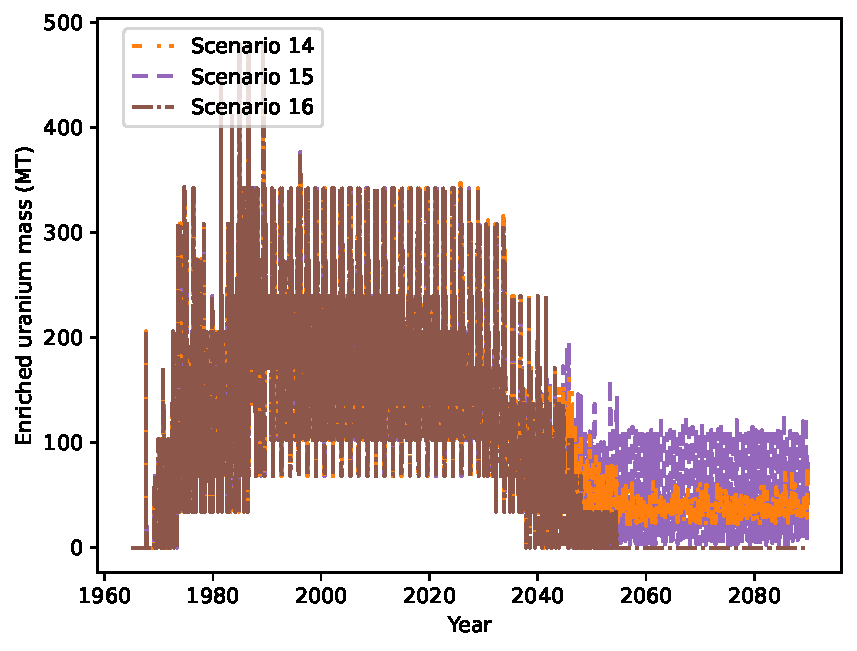
\includegraphics[width=\textwidth]{nogrowth_recycle_total_fuel.pdf}
        \caption{Monthly mass of enriched uranium sent to all reactors 
        between 1965-2090.}
        \label{fig:nogrowth_recycle_all_uranium}
    \end{subfigure}
    \hfill
    \begin{subfigure}[b]{0.45\textwidth}
        \centering
        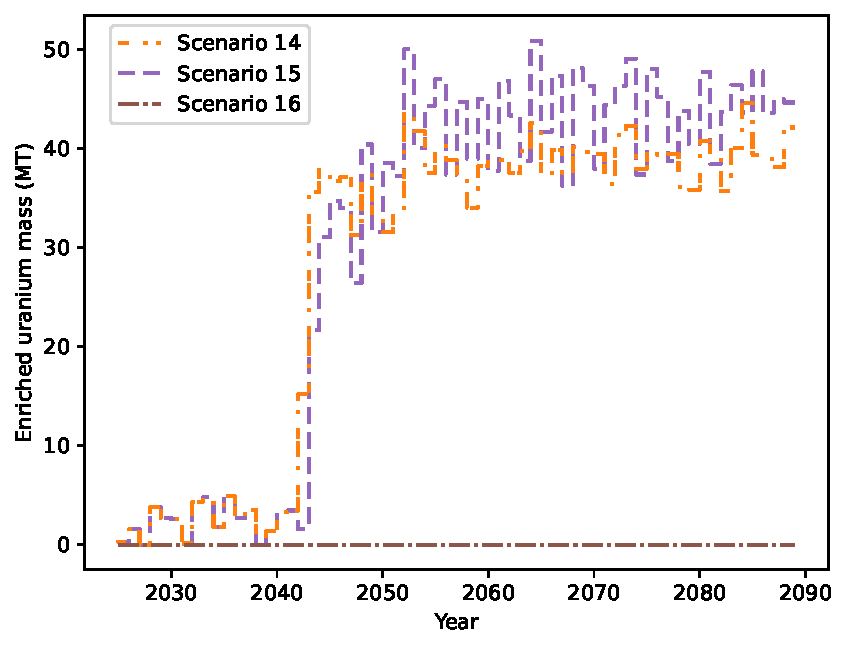
\includegraphics[width=\textwidth]{nogrowth_recycle_Uaverages.pdf}
        \caption{Annual average mass of enriched uranium sent to 
        advanced reactors between 2025-2090.}
        \label{fig:nogrowth_recycle_AR_uranium}
    \end{subfigure}
    \begin{subfigure}[b]{0.45\textwidth}
        \centering
        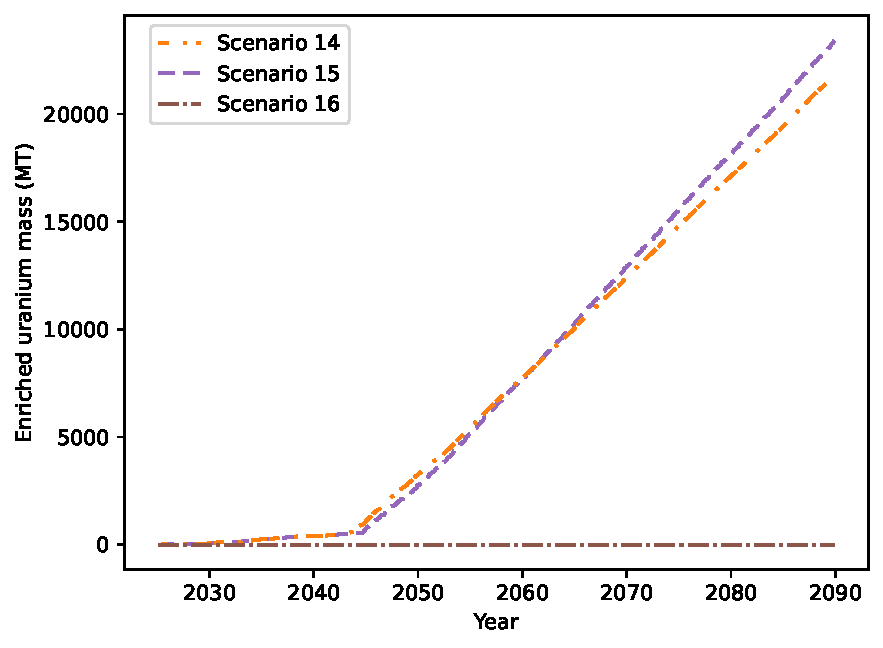
\includegraphics[width=\textwidth]{nogrowth_recycle_Ucumulative.pdf}
        \caption{Cumulative mass of enriched 
        uranium sent to advanced reactors between 2025-2090.}
        \label{fig:nogrowth_recycle_uranium_cumulative}
    \end{subfigure}
       \caption{Mass of enriched uranium required by reactors
        in Scenarios 14-16.}
       \label{fig:nogrowth_recycle_uranium}
\end{figure}

Scenario 15 requires the most enriched 
uranium because less material is available for reprocessing, leading to 
less separated plutonium and less \gls{MOX} fuel available. 
The annual average mass of enriched uranium in Scenarios 14 and 15 increases 
in 2043 because the \gls{MOX} stockpiled up from the \gls{LWR} \gls{SNF} 
is used up and there is not as much plutonium from the advanced reactor 
\gls{SNF} to produce more \gls{MOX} fuel. 

Scenario 16 does not require any uranium-based fuel to support the 
advanced reactors. This result stems from a few key differences between 
these fuel cycles. The first difference is that all of the advanced 
reactors in Scenario 16 can accept reprocessed fuel, while the \glspl{MMR} 
in Scenarios 14 and 15 will only accept \gls{UOX}. This modeling 
decision for the \gls{MMR} means that any fuel cycle that 
deploys the \gls{MMR} will always require some amount of uranium-based 
fuel. The second is the reprocessing scheme.  
In Scenario 16, the spent fuel can be reprocessed an infinite number 
of times while in Scenarios 14 and 15 the spent uranium-based fuel can 
only be reprocessed once and the plutonium-based fuel can not be 
reprocessed. This difference is inherent to the type of fuel cycle 
(limited vs. continuous recycle). Additionally, the reprocessing 
step in Scenario 16 removes the uranium, neptunium, plutonium, 
and americium from the spent fuel, compared with only plutonium 
being separated out in Scenarios 14 and 15. The unlimited number of 
times the spent fuel can be reprocessed and the additional 
elements separated out in Scenario 16 increases the amount of 
reprocessed fuel available.

Table \ref{tab:s14-16_uranium} reports the average enriched uranium mass, 
average \gls{HALEU} mass, maximum enriched uranium mass, and cumulative 
enriched uranium mass required by these scenarios. Scenario 14 requires 
less enriched uranium than Scenario 7, despite having the same 
advanced reactor deployment schedule, because of the change in the 
fuel cycle. By reprocessing spent fuel, the average \gls{HALEU} 
mass required drops by 21.3\%. A similar decrease in cumulative 
\gls{HALEU} needs is seen in Scenario 15, but the removal of 
\gls{TRISO} reprocessing results in a smaller decrease (15.1\%
decrease). By reprocessing the \gls{TRISO}-based fuels in 
Scenario 14, this scenario needs to a 6.35\% reduction in the 
cumulative enriched uranium needs from Scenario 15. 

\begin{table}[h!]
    \centering 
    \caption{Metrics for enriched uranium required to fuel reactors 
    in Scenarios 14-16.}
    \label{tab:s14-16_uranium}
    \begin{tabular}{c c c c c}
        \hline 
        Scenario & Average (MT/month) & HALEU Average (MT/month) 
        & Maximum (MT) & Cumulative (MT) \\
        \hline 
        14 & 28.01 & 27.16 & 87.01 & 21,920 \\
        15 & 30.05 & 29.20 & 143.8 & 23,407\\
        16 & 0 & 0 & 0 & 0\\
        \hline
        
    \end{tabular}
\end{table}

In addition to the enriched uranium, the advanced 
reactors receive heavy metals for the plutonium-based 
fuels. Figure 
\ref{fig:nogrowth_recycle_mox} shows that Scenario 16 requires more 
plutonium-based fuel than the other scenarios. This result is consistent 
with the reactors in Scenarios 16 not receiving any enriched 
uranium. As Table 
\ref{tab:s14-16_mox} reports, Scenario 16 needs a monthly average 
of plutonium-based fuel that is larger than the maximum mass 
needed in Scenarios 14 and 15. More heavy metal for plutonium-based fuel
is sent to advanced reactor in Scenario 14 than  
in Scenario 15 because of the greater availability of 
\gls{MOX} fuel from the additional reprocessing of 
\gls{TRISO}-based fuel. The heavy metals for plutonium fuels 
in Scenarios 14 and 15 show a decrease in 2043, corresponding 
to the increase in enriched uranium sent to reactors in these 
scenarios. After the initial stock of \gls{MOX} from 
\gls{LWR} spent fuel is used in Scenarios 14 and 15, an 
average of 5.26 MT/month and 1.49 MT/month, respectively. These 
values are both smaller than the average values reported 
in Table \ref{tab:s14-16_mox}, highlighting the importance 
of a stockpile of \gls{MOX} from \gls{LWR} spent fuel in 
providing \gls{MOX} for advanced reactors in these fuel 
cycles. 

\begin{figure}[h!]
    \centering
    \begin{subfigure}[b]{0.45\textwidth}
        \centering
        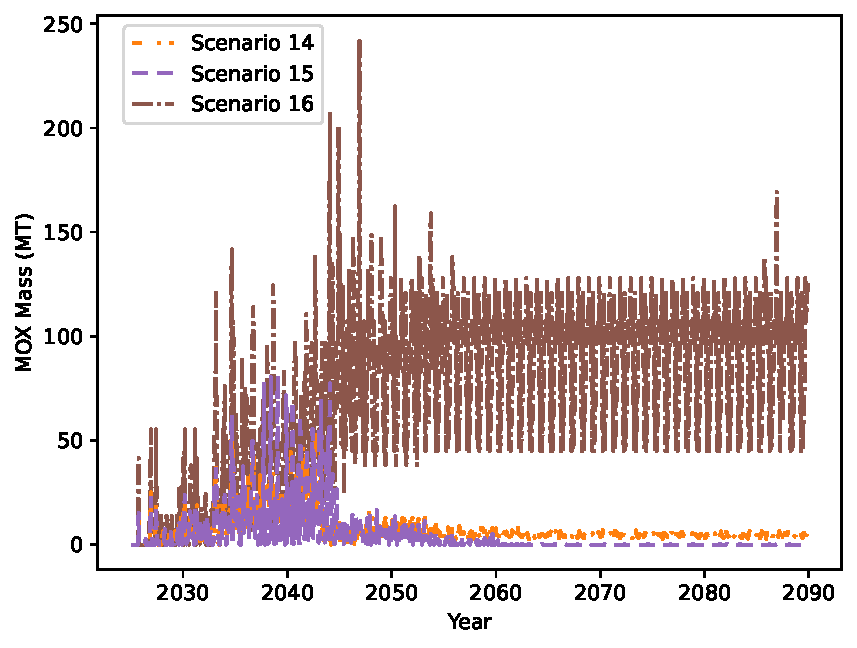
\includegraphics[width=\textwidth]{nogrowth_recycle_MOX.pdf}
        \caption{Monthly masses of plutonium-based fuel sent to 
        advanced reactors between 2025-2090.}
        \label{fig:nogrowth_recycle_AR_mox}
    \end{subfigure}
    \hfill
    \begin{subfigure}[b]{0.45\textwidth}
        \centering
        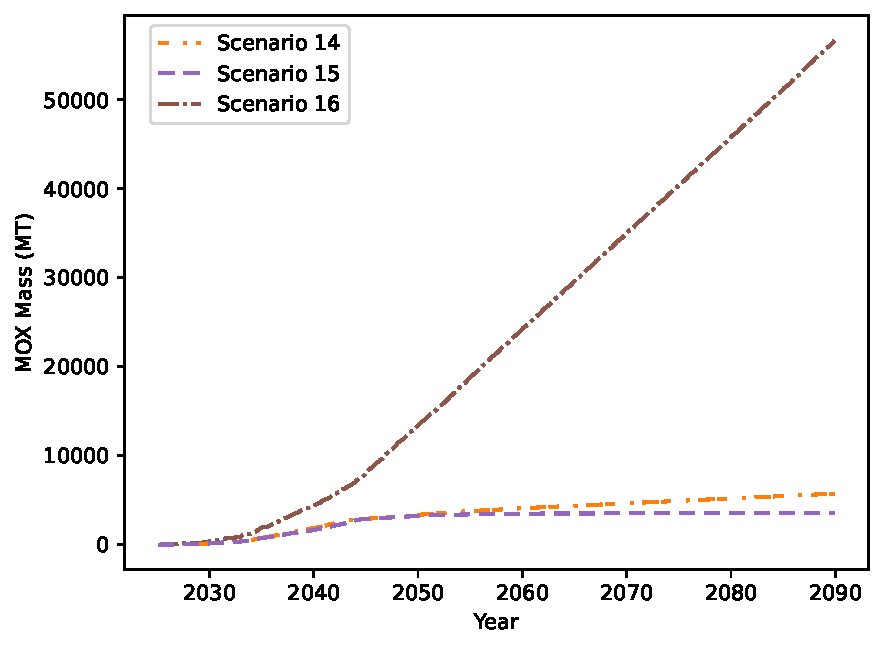
\includegraphics[width=\textwidth]{nogrowth_recycle_MOXcumulative.pdf}
        \caption{Cumulative mass of plutonium-based fuel
        sent to advanced reactors between 2025-2090.}
        \label{fig:nogrowth_recycle_mox_cumulative}
    \end{subfigure}
       \caption{Mass of plutonium-based fuel required by reactors
        in Scenarios 14-16.}
       \label{fig:nogrowth_recycle_mox}
\end{figure}

\begin{table}[h!]
    \centering 
    \caption{Metrics for plutonium-based fuels required to fuel reactors 
    in Scenarios 14-16.}
    \label{tab:s14-16_mox}
    \begin{tabular}{c c c c}
        \hline 
        Scenario & Average (MT/month) & Maximum (MT) & Cumulative (MT) \\
        \hline 
        14 & 7.351 & 53.81 & 5,727 \\
        15 & 4.506 & 81.59 & 3,510 \\
        16 & 72.70 & 241.9 & 56,630 \\
        \hline
        
    \end{tabular}
\end{table}

When comparing the total cumulative mass of heavy metal (enriched 
uranium and heavy metal in plutonium-based fuel) required by each scenario,
Scenario 16 needs the most material of these three scenarios. This 
result stems from the different discharge burnups of the reactors. The 
\gls{SFR} has a burnup of 87.51 MWd/kg HM and the Xe-100 (the reactor that 
meets most of the demand in Scenarios 14 and 15) has a burnup of 168 MWd/kg U. 
The Xe-100 gets more energy out of each unit mass of fuel, which leads to 
Scenarios 14 and 15 requiring less fuel than Scenario 16. Scenario 16 is most 
similar to Scenario 2 in the amount of heavy metals required. This result 
stems from the \gls{SFR} and \gls{MMR} having similar discharge burnups.

\subsubsection{Natural uranium}
The natural uranium required as feed uranium to produce enriched 
uranium fuel for reactors is shown in Figure \ref{fig:nogrowth_recycle_feed}, 
and the metrics reported in Table \ref{tab:s14-16_feed}. Scenario 15 requires 
the most feed uranium, followed by Scenarios 14 and 16. This pattern follows 
with the enriched uranium mass in each scenario. Scenario 15 requires the 
most feed mass because less spent fuel is reprocessed, leading to more 
enriched uranium required, leading to more feed uranium needed. Scenario 
16 does not requires any feed uranium because it does not require any 
enriched uranium. The cumulative feed uranium needed in Scenarios 14 and 
15 are both less than the cumulative feed uranium needed in Scenario 7.

\begin{figure}[h!]
    \centering
    \begin{subfigure}[b]{0.45\textwidth}
        \centering
        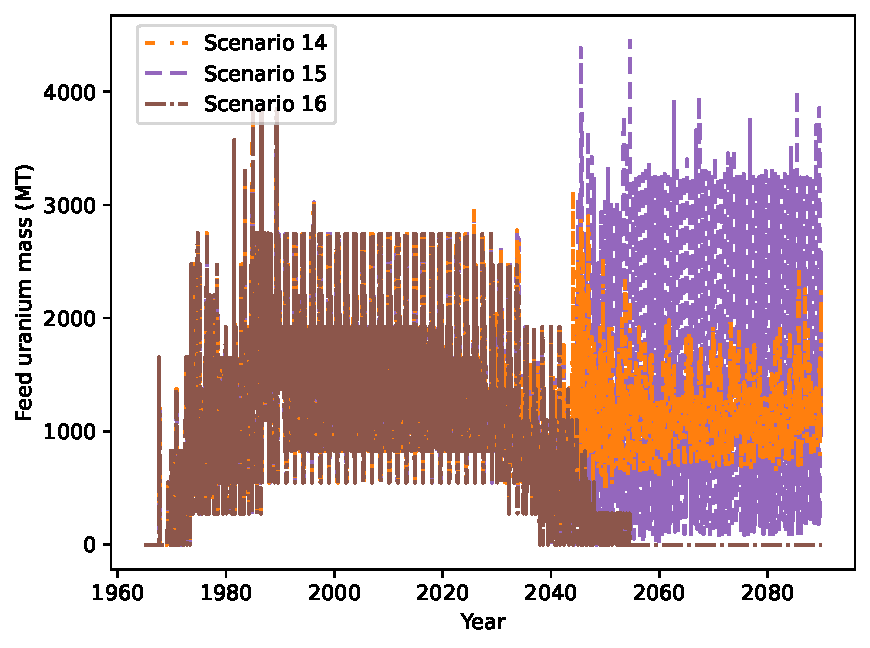
\includegraphics[width=\textwidth]{nogrowth_recycle_feed.pdf}
        \caption{Monthly mass 
        for all reactors between 1965-2090.}
        \label{fig:nogrowth_recycle_all_feed}
    \end{subfigure}
    \hfill
    \begin{subfigure}[b]{0.45\textwidth}
        \centering
        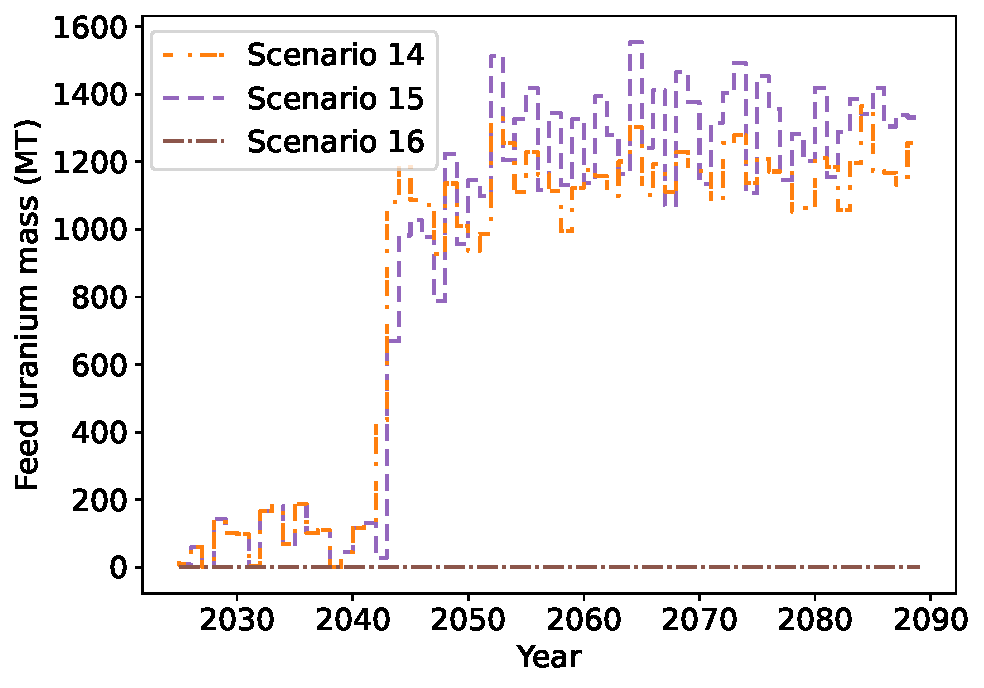
\includegraphics[width=\textwidth]{nogrowth_recycle_feed_average.pdf}
        \caption{Annual average  mass 
        for all reactors between 2025-2090.}
        \label{fig:nogrowth_recycle_AR_feed}
    \end{subfigure}
    \begin{subfigure}[b]{0.45\textwidth}
        \centering
        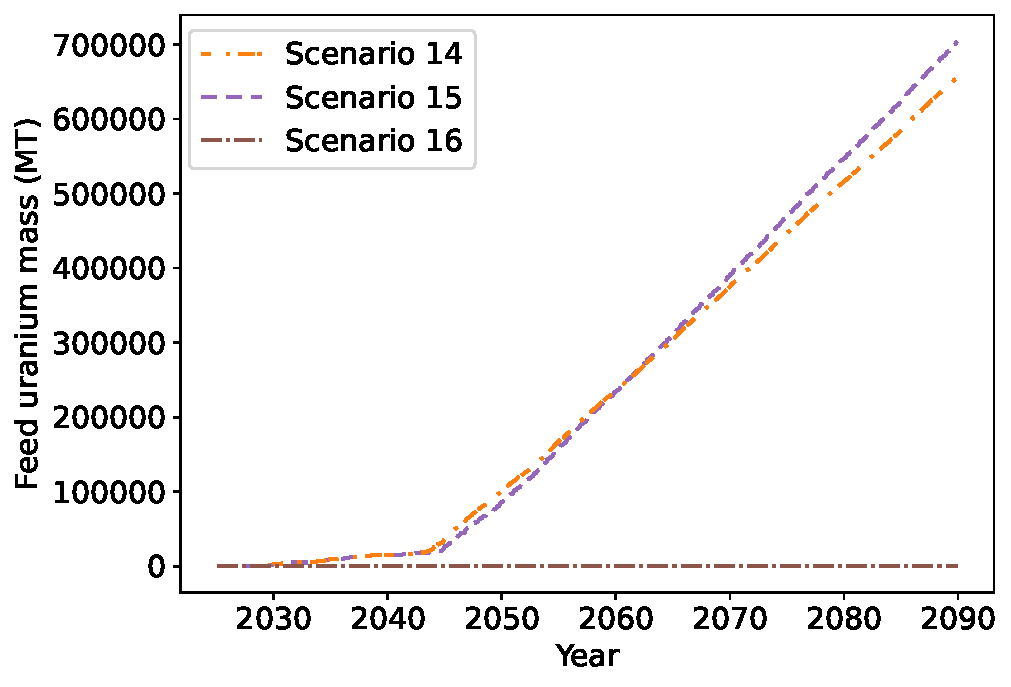
\includegraphics[width=\textwidth]{nogrowth_recycle_feed_cumulative.pdf}
        \caption{Cumulative mass sent to advanced reactors between 2025-2090.}
        \label{fig:nogrowth_recycle_feed_cumulative}
    \end{subfigure}
       \caption{Mass of enriched uranium required by reactors
        in Scenarios 14-16.}
       \label{fig:nogrowth_recycle_feed}
\end{figure}

\begin{table}[h!]
    \centering 
    \caption{Metrics for feed uranium required to produce 
    uranium-based fuels in in Scenarios 14-16.}
    \label{tab:s14-16_feed}
    \begin{tabular}{c c c c c}
        \hline 
        Scenario & Average (MT/month) & HALEU Average (MT/month) &
        Maximum (MT) & Cumulative (MT) \\
        \hline 
        14 & 842.9 & 836.4 & 2,628 & 656,582 \\
        15 & 903.9 & 897.4 & 4,450 & 704,106\\
        16 & 0 & 0 & 0 & 0\\
        \hline
        
    \end{tabular}
\end{table}

Next, Figure \ref{fig:nogrowth_recycle_natu} shows the natural 
uranium required for the plutonium-based fuels in Scenarios 14-16. 
These results follow the same pattern as the heavy metal for 
plutonium-based fuels in these scenarios. Scenario 16 requires 
the most natural uranium because the reactors in this scenario 
only receive the U/TRU fuel. Scenario 15 requires the least 
natural uranium, because this scenario results in the least 
plutonium-based fuel.

\begin{figure}[h!]
    \centering
    \begin{subfigure}[b]{0.45\textwidth}
        \centering
        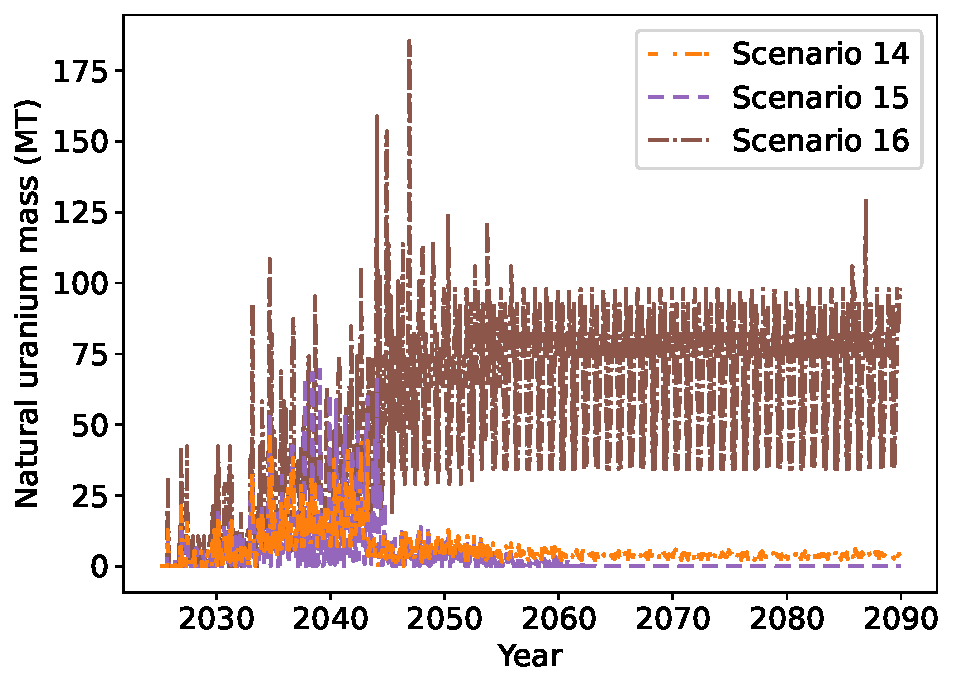
\includegraphics[width=\textwidth]{nogrowth_recycle_natU.pdf}
        \caption{Monthly masses sent to 
        advanced reactors between 2025-2090.}
        \label{fig:nogrowth_recycle_AR_natu}
    \end{subfigure}
    \hfill
    \begin{subfigure}[b]{0.45\textwidth}
        \centering
        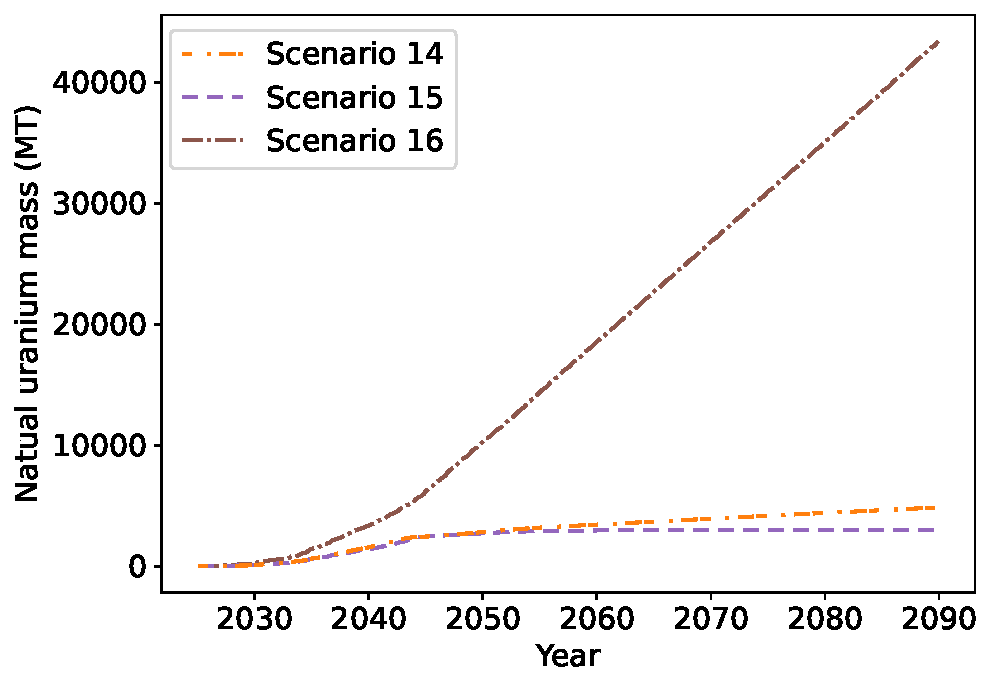
\includegraphics[width=\textwidth]{nogrowth_recycle_natU_cumulative.pdf}
        \caption{Cumulative mass of between 2025-2090.}
        \label{fig:nogrowth_recycle_natu_cumulative}
    \end{subfigure}
       \caption{Mass of natural uranium for plutonium-based fuel required 
       by reactors
        in Scenarios 14-16.}
       \label{fig:nogrowth_recycle_natu}
\end{figure}

Table \ref{tab:s14-16_natU} reports the metrics fo the natural uranium 
required for Scenarios 14-16. The cumulative natural uranium mass 
needed by Scenario 16 is more than one order of magnitude smaller than 
the cumulative feed uranium masses in Scenarios 14 and 15. This 
decrease in masses is because using natural uranium for plutonium-based 
fuels does not have the same process losses as using the 
material as feed material for enrichment. This result suggests that 
using a closed fuel cycle, and more specifically using a continuous 
reprocessing fuel cycle, is ideal for limiting the natural uranium 
needed in a fuel cycle. 

\begin{table}[h!]
    \centering 
    \caption{Metrics for natural uranium required to produce 
    plutonium-based fuels in Scenarios 14-16.}
    \label{tab:s14-16_natU}
    \begin{tabular}{c c c c}
        \hline 
        Scenario & Average (MT/month) & Maximum (MT) & Cumulative (MT) \\
        \hline 
        14 & 6.256 & 45.80 & 4,874 \\
        15 & 3.835 & 69.44 & 2,987 \\
        16 & 55.68 & 185.3 & 43,372 \\
        \hline
        
    \end{tabular}
\end{table}

\subsection{1\% growth scenarios}
This section presents the results of the uranium resources required 
in the 1\% growth, closed fuel cycle scenarios (Scenarios 17-19). 
These results are split into the fuel masses (enriched uranium 
and heavy metals in plutonium-based fuel) and the natural 
uranium masses (feed uranium and natural uranium to produce 
plutonium-based fuels).

\subsubsection{Fuel masses}
The first fuel mass we consider is the enriched uranium mass, 
shown in Figure \ref{fig:1percent_recycle_uranium}. These results 
show the same pattern as this metric for the no growth scenarios:
Scenario 18 requires the most enriched uranium and Scenario 19 
does not require any enriched uranium. In Scenarios 17 and 18 the 
increase in enriched uranium need occurs closer to 2040 and is a 
more gradual increase. These results stem from the growth in energy 
demand, and subsequently reactor deployment, leading to the stockpile 
of \gls{MOX} from \gls{LWR} spent fuel to be used up sooner. 
Additionally, the change in reactor deployment leads to different 
proportions of the advanced reactors, which leads to the more gradual 
increase in the enriched uranium needs. There is also an increase in 
the enriched uranium sent to reactors in Scenario 17 
around 2085. This increased demand comes from ???

\begin{figure}[h!]
    \centering
    \begin{subfigure}[b]{0.45\textwidth}
        \centering
        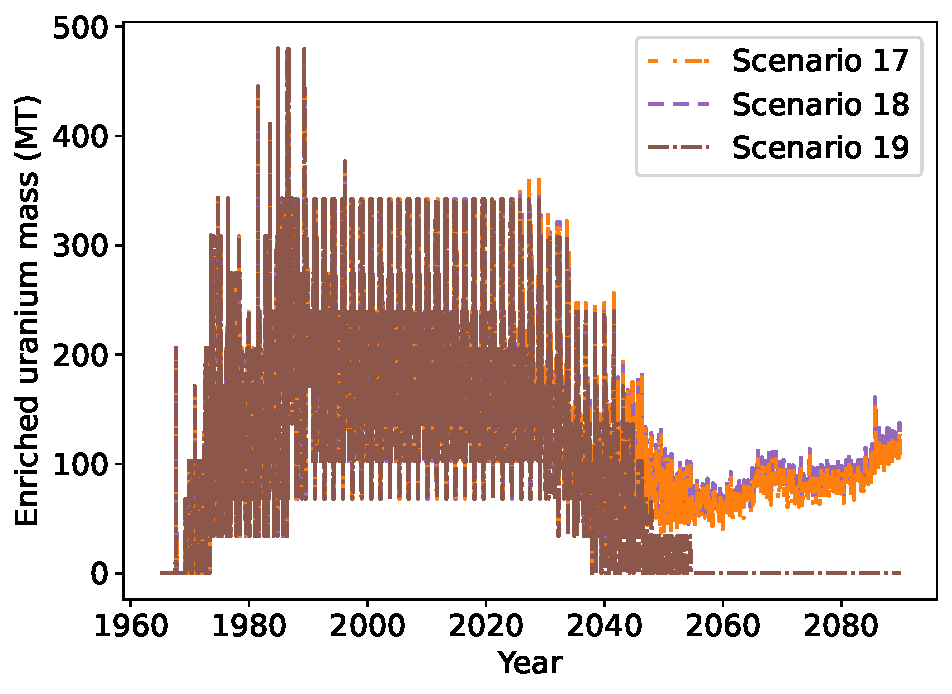
\includegraphics[width=\textwidth]{1percent_recycle_total_fuel.pdf}
        \caption{Monthly mass of enriched uranium sent to all reactors 
        between 1965-2090.}
        \label{fig:1percent_recycle_all_uranium}
    \end{subfigure}
    \hfill
    \begin{subfigure}[b]{0.45\textwidth}
        \centering
        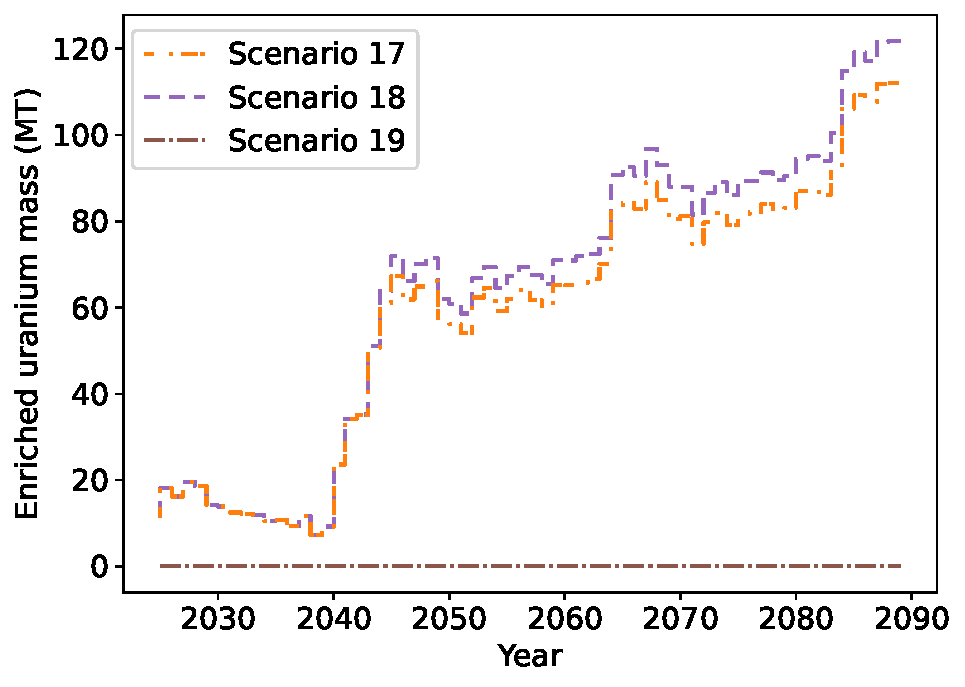
\includegraphics[width=\textwidth]{1percent_recycle_Uaverages.pdf}
        \caption{Annual average mass of enriched uranium sent to 
        advanced reactors between 2025-2090.}
        \label{fig:1percent_recycle_AR_uranium}
    \end{subfigure}
    \begin{subfigure}[b]{0.45\textwidth}
        \centering
        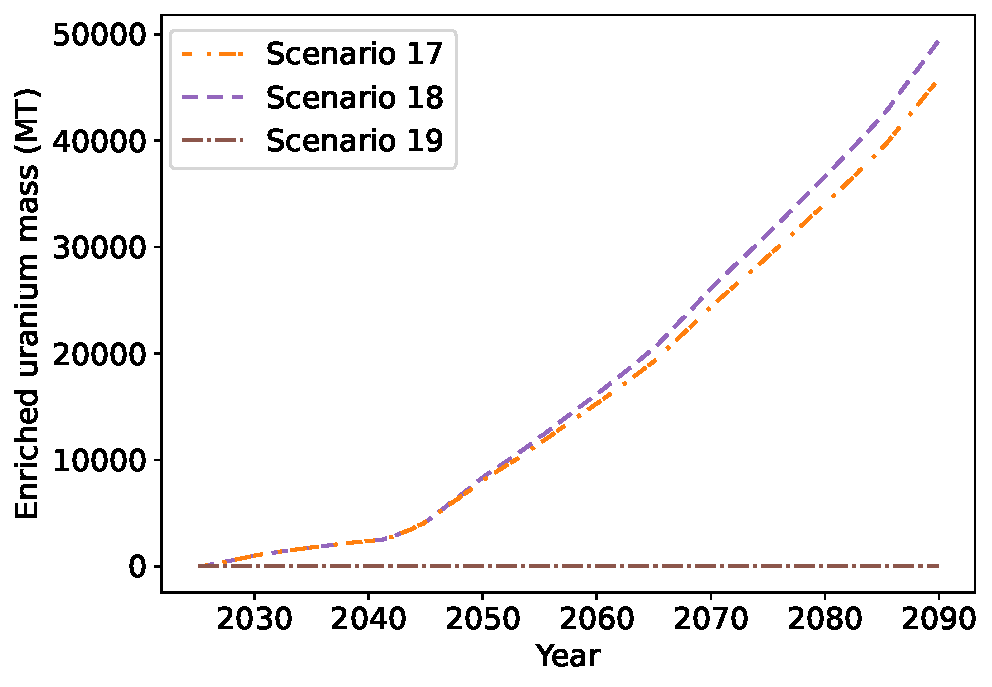
\includegraphics[width=\textwidth]{1percent_recycle_Ucumulative.pdf}
        \caption{Cumulative mass of enriched 
        uranium sent to advanced reactors between 2025-2090.}
        \label{fig:1percent_recycle_uranium_cumulative}
    \end{subfigure}
       \caption{Mass of enriched uranium required by reactors
        in Scenarios 17-19.}
       \label{fig:1percent_recycle_uranium}
\end{figure}

Table \ref{tab:s17-19_enrichedU} reports the metrics for the enriched 
uranium masses for Scenarios 17-19. The cumulative enriched 
uranium in Scenarios 17 and 18 are less than the cumulative 
enriched uranium required by Scenario 13. However, the cumulative 
mass for Scenario 18 is larger than the cumulative in Scenario 
9. These results highlight how reprocessing can reduce enriched 
uranium needs, but the reactors deployed and their fuel usage 
is still an important factor in how much enriched uranium is 
needed. 

\begin{table}[h!]
    \centering 
    \caption{Metrics of enriched uranium fuel between 2025-2090 in Scenarios 
    17-19.}
    \label{tab:s17-19_enrichedU}
    \begin{tabular}{c c c c c}
        \hline 
        Scenario & Average (MT/month) & Average HALEU (MT/month) &  
        Maximum (MT) & Cumulative (MT) \\
        \hline
        17 & 50.81 & 45.67 & 384.3 & 39,582\\
        18 & 63.32 & 57.42 & 160.9 & 49,329\\
        19 & 0 & 0 & 0 & 0\\
        \hline
    \end{tabular}
\end{table}

Next is the mass of plutonium-based fuels sent to the advanced reactors 
in Scenarios 17-19, shown in Figure \ref{fig:1percent_recycle_mox}.
Similar to the no growth scenarios, Scenario 19 requires the most 
plutonium-based fuel of the three scenarios and Scenario 17 
requires more than Scenario 18. Scenarios 17 and 18 show the 
initial stockpile of \gls{MOX} from \gls{LWR} spent fuel that 
gets used by 2040. 

\begin{figure}[h!]
    \centering
    \begin{subfigure}[b]{0.45\textwidth}
        \centering
        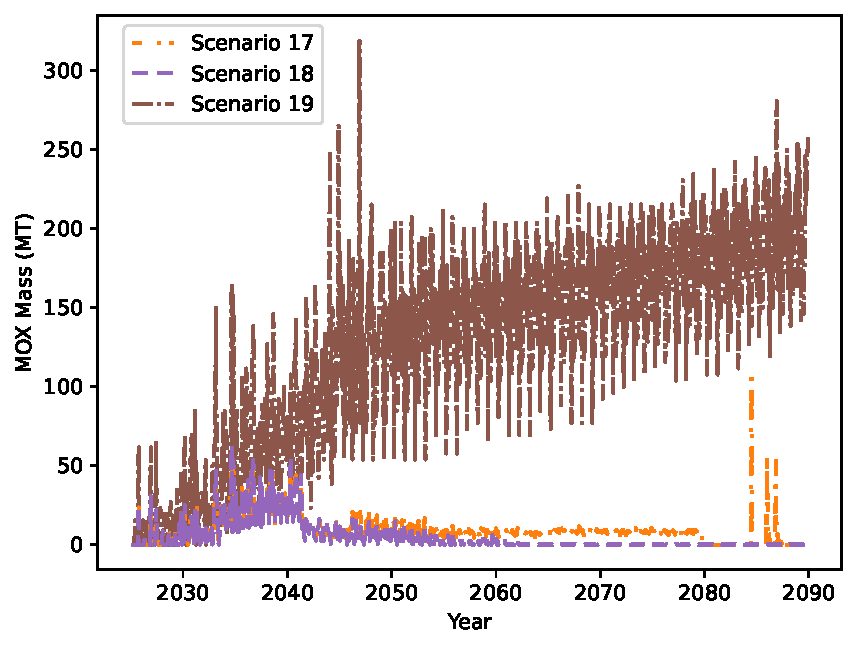
\includegraphics[width=\textwidth]{1percent_recycle_MOX.pdf}
        \caption{Monthly mass of sent to all reactors 
        between 1965-2090.}
        \label{fig:1percent_recycle_AR_mox}
    \end{subfigure}
    \hfill
    \begin{subfigure}[b]{0.45\textwidth}
        \centering
        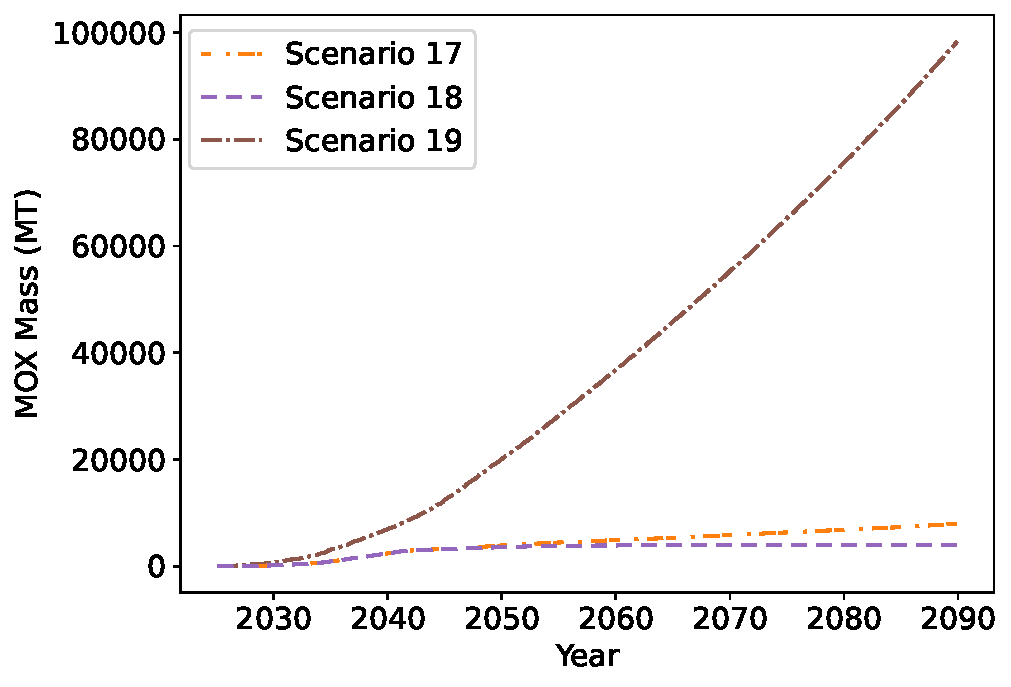
\includegraphics[width=\textwidth]{1percent_recycle_MOXcumulative.pdf}
        \caption{Cumulative mass  
        sent to advanced reactors between 2025-2090.}
        \label{fig:1percent_recycle_mox_cumulative}
    \end{subfigure}
       \caption{Masses of plutonium-based fuel sent to advanced reactors
        in Scenarios 17-19.}
       \label{fig:1percent_recycle_mox}
\end{figure}

Table \ref{tab:s17-19_mox} reports the metrics for the plutonium-based 
fuels in Scenarios 17-19. Scenario 19 requires more heavy metal (in enriched 
uranium and plutonium-based fuels) than Scenarios 
17 and 18, as Scenarios 9, 10, 12, and 13. This result shows how the 
the reactors deployed play an important role in determining how 
much fuel is required for a fuel cycle.  

\begin{table}[h!]
    \centering 
    \caption{Metrics of plutonium-based fuel between 2025-2090 in Scenarios 
    17-19.}
    \label{tab:s17-19_mox}
    \begin{tabular}{c c c c}
        \hline 
        Scenario & Average (MT/month) & Maximum (MT) & Cumulative (MT) \\
        \hline
        17 & 9.077 & 106.1 & 7,071\\
        18 & 5.109 & 62.56 & 3,979\\
        19 & 126.2 & 318.7 & 98,323\\
        \hline
    \end{tabular}
\end{table}

\subsubsection{Natural uranium}
The next two metrics are related to the natural uranium requirements of 
the 1\% growth scenarios. The first of these two metrics is the 
natural uranium needed as feed material for enrichment, shown in 
Figure \ref{fig:1percent_recycle_feed}. The feed uranium masses follow with 
the enriched uranium masses in these scenarios. Scenario 18 requires 
the most feed uranium, and Scenario 19 requires no feed uranium. 

\begin{figure}[h!]
    \centering
    \begin{subfigure}[b]{0.45\textwidth}
        \centering
        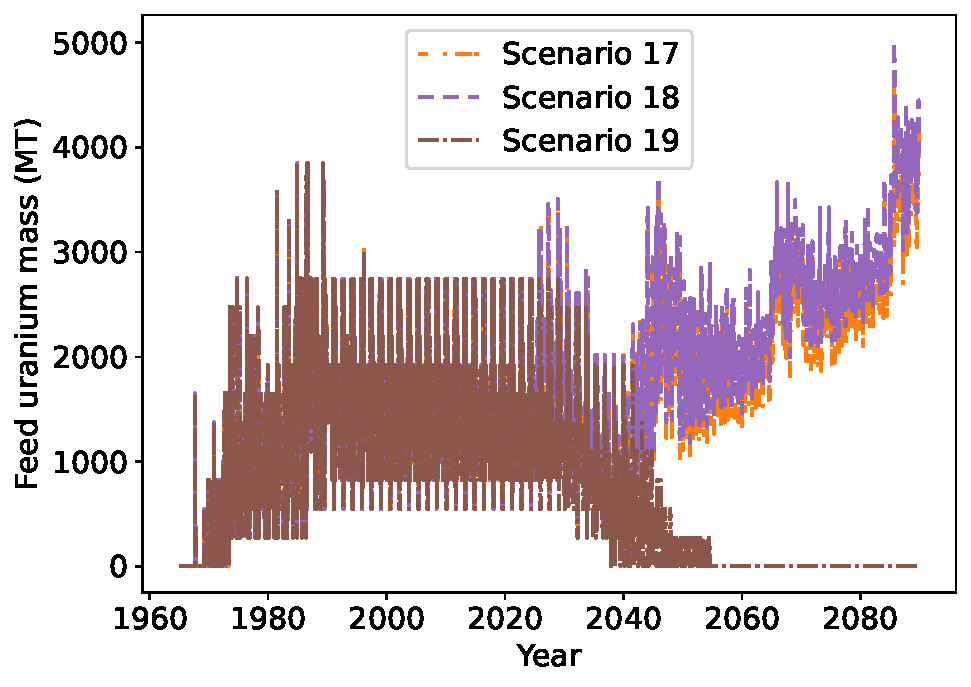
\includegraphics[width=\textwidth]{1percent_recycle_feed.pdf}
        \caption{Monthly mass for all reactors 
        between 1965-2090.}
        \label{fig:1percent_recycle_all_feed}
    \end{subfigure}
    \hfill
    \begin{subfigure}[b]{0.45\textwidth}
        \centering
        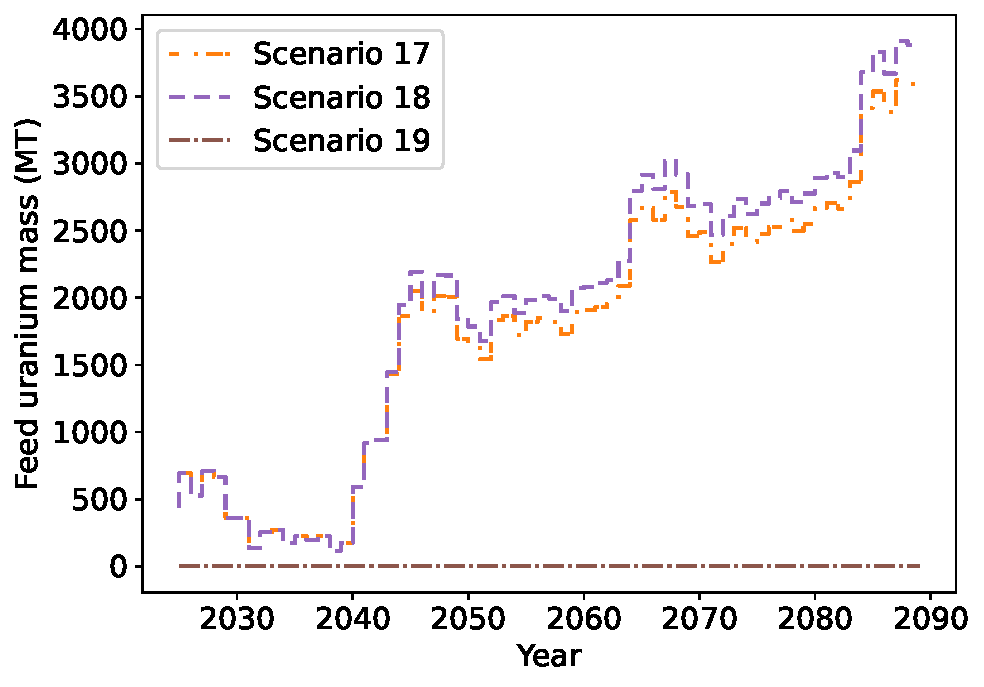
\includegraphics[width=\textwidth]{1percent_recycle_feed_average.pdf}
        \caption{Annual average mass for 
        advanced reactors between 2025-2090.}
        \label{fig:1percent_recycle_AR_feed}
    \end{subfigure}
    \begin{subfigure}[b]{0.45\textwidth}
        \centering
        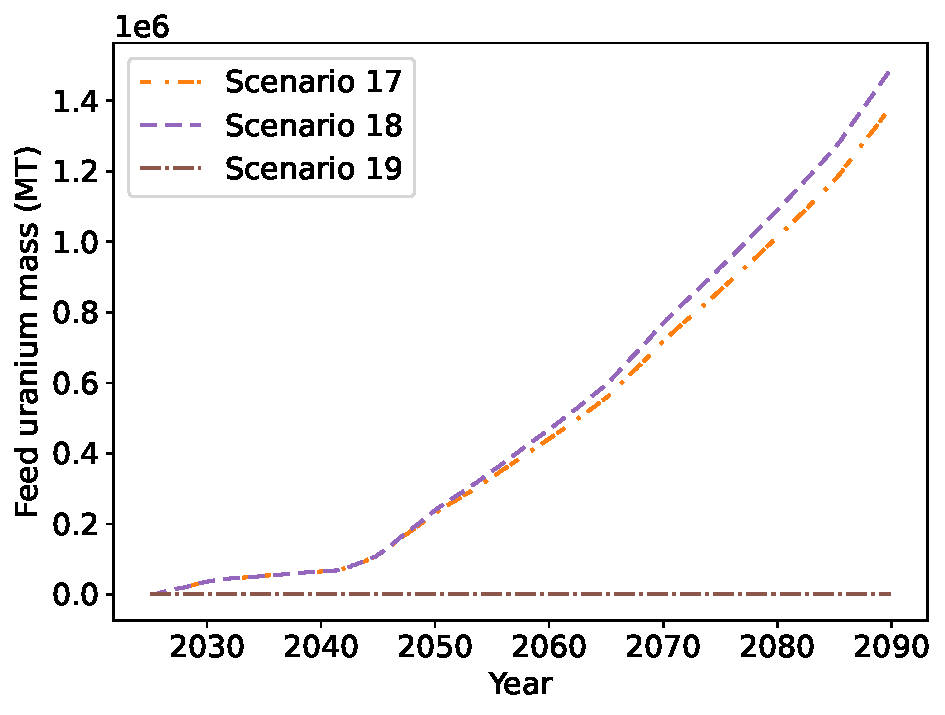
\includegraphics[width=\textwidth]{1percent_recycle_feed_cumulative.pdf}
        \caption{Cumulative mass for advanced reactors between 2025-2090.}
        \label{fig:1percent_recycle_feed_cumulative}
    \end{subfigure}
       \caption{Masses of feed uranium required by reactors
        in Scenarios 17-19.}
       \label{fig:1percent_recycle_feed}
\end{figure}

Table \ref{tab:s17-19_feed} reports the metrics for the feed uranium in 
Scenarios 17-19. Scenarios 17 and 18 need less feed uranium than 
Scenario 13, for all of the metrics except the maximum in Scenario 17. 
Scenario 17 requires more feed uranium than Scenario 9, and 
Scenario 18 requires more feed uranium than Scenarios 9 and 12. 

\begin{table}[h!]
    \centering 
    \caption{Metrics of feed uranium to produce enriched uranium 
    between 2025-2090 in Scenarios 17-19.}
    \label{tab:s17-19_feed}
    \begin{tabular}{c c c c c}
        \hline 
        Scenario & Average (MT/month) & HALEU Average (MT/month) & 
        Maximum (MT) & Cumulative (MT) \\
        \hline
        17 & 1,553 & 1,514 & 11,435 & 1,210,540\\
        18 & 1,866 & 1,911 & 5,014 & 1,489,022\\
        19 & 0 & 0 & 0 & 0\\
        \hline
    \end{tabular}
\end{table}

Finally, Figure \ref{fig:1percent_recycle_natU} shows the natural uranium 
required to produce plutonium-based fuels in Scenarios 17-19. 

\begin{figure}[h!]
    \centering
    \begin{subfigure}[b]{0.45\textwidth}
        \centering
        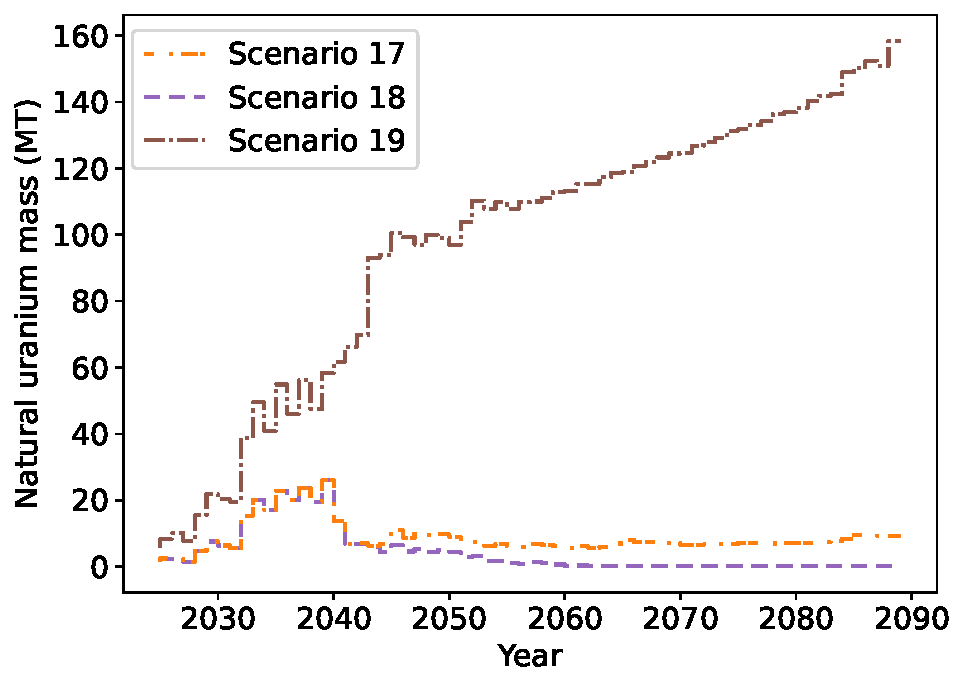
\includegraphics[width=\textwidth]{1percent_recycle_natU.pdf}
        \caption{Monthly mass sent to all reactors 
        between 1965-2090.}
        \label{fig:1percent_recycle_AR_natu}
    \end{subfigure}
    \hfill
    \begin{subfigure}[b]{0.45\textwidth}
        \centering
        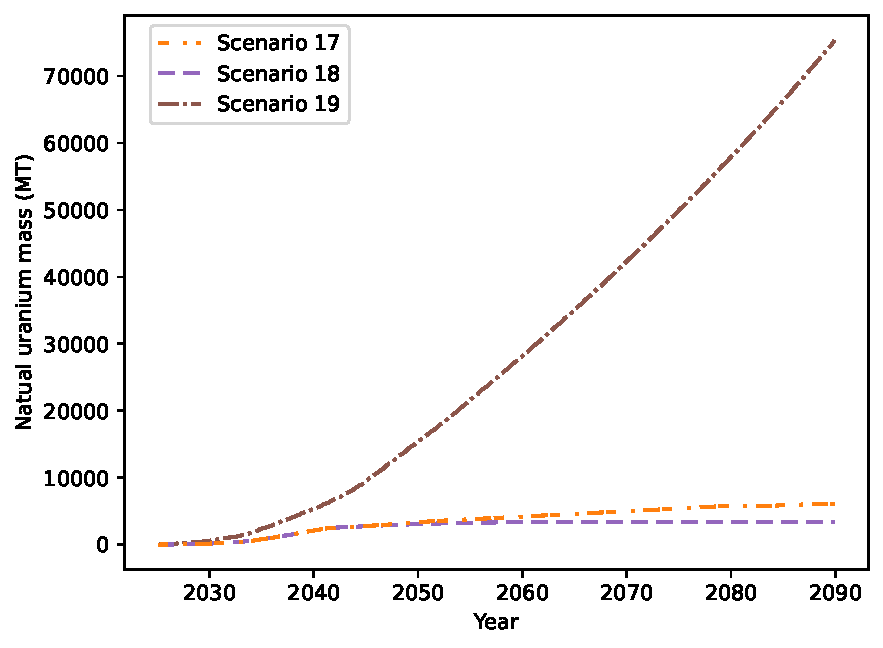
\includegraphics[width=\textwidth]{1percent_recycle_natU_cumulative.pdf}
        \caption{Cumulative mass  sent to 
        advanced reactors between 2025-2090.}
        \label{fig:1percent_recycle_natu_cumulative}
    \end{subfigure}
       \caption{Mass of natural uranium required by reactors
        in Scenarios 17-19.}
       \label{fig:1percent_recycle_natU}
\end{figure}

Table \ref{tab:s17-19_natU} reports the metrics for the 
natural uranium for plutonium-based fuels in Scenarios 17-19. 

\begin{table}[h!]
    \centering 
    \caption{Metrics of natural uranium required to produce 
    plutonium-based fuel between 2025-2090 in Scenarios 
    17-19.}
    \label{tab:s17-19_natU}
    \begin{tabular}{c c c c}
        \hline 
        Scenario & Average (MT/month) & Maximum (MT) & Cumulative (MT) \\
        \hline
        17 &  &  & \\
        18 &  &  & \\
        19 &  &  & \\
        \hline
    \end{tabular}
\end{table}


\section{SWU capacity}
The next category of metrics of interest is the \gls{SWU} capacity required 
to produce the enriched uranium in each of the scenarios. The \gls{SWU} 
capacity has important implications on the enrichment facilities required 
to support these fuel cycles. 

\subsection{No growth scenarios}
Figure \ref{fig:nogrowth_recycle_swu} shows \gls{SWU} capacity required 
in Scenarios 14-16. For Scenarios 14 and 15 the required \gls{SWU} 
capacity for the advanced reactors is relatively small, then increases 
around 2043, corresponding with the increased need for enriched uranium 
for reactors in these scenarios. 
\begin{figure}[h!]
    \centering
    \begin{subfigure}[b]{0.45\textwidth}
        \centering
        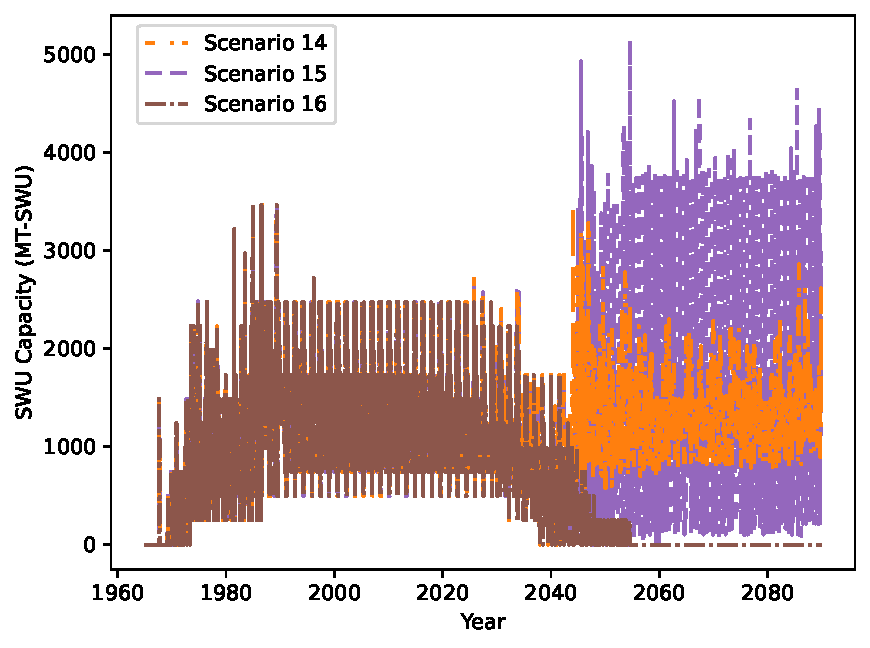
\includegraphics[width=\textwidth]{nogrowth_recycle_swu.pdf}
        \caption{Monthly SWU capacity required to produce 
        enriched uranium for all reactors between 2025-2090.}
        \label{fig:nogrowth_recycle_swu_all}
    \end{subfigure}
    \hfill
    \begin{subfigure}[b]{0.45\textwidth}
        \centering
        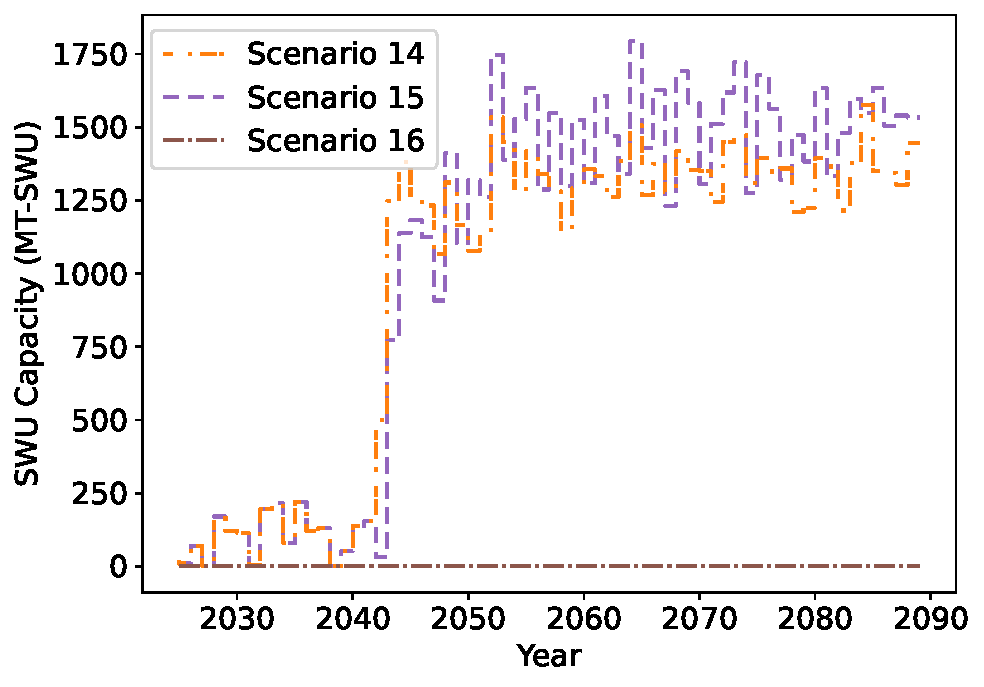
\includegraphics[width=\textwidth]{nogrowth_recycle_AR_swu.pdf}
        \caption{Monthly SWU capacity required to produce 
        enriched uranium for advanced reactors between 2025-2090.}
        \label{fig:nogrowth_recycle_swu_AR}
    \end{subfigure}
       \caption{\gls{SWU} capacity required in Scenarios 14-16.}
       \label{fig:nogrowth_recycle_swu}
\end{figure}

Table \ref{tab:s14-16_swu} reports the metrics of required \gls{SWU} 
capacity in Scenarios 14-16. Scenarios 14 and 15 require smaller 
average \gls{SWU} capacities than Scenarios 2-7, and require a 
smaller average \gls{SWU} capacity to produce \gls{HALEU} than 
Scenarios 2, 3, 4, 6, and 7. Scenario 5 requires less \gls{SWU} 
capacity to produce \gls{HALEU} because this scenario 
primarily deploys VOYGRs. Scenario 16 requires the least 
\gls{SWU} capacity of any of the no growth transitions 
modeled in this work, because the \glspl{SFR} in this scenario
do not receive any enriched uranium. The differences in the 
\gls{SWU} capacity needed by these scenarios is a function of 
the reactors deployed and the amount of material available for 
reprocessing.

\begin{table}[h!]
    \centering 
    \caption{Metrics for \gls{SWU} capacity required to produce 
    enriched uranium in Scenarios 14-16.}
    \label{tab:s14-16_swu}
    \begin{tabular}{c c c c}
        \hline 
        Scenario & Average (MT-SWU/month) & HALEU Average (MT-SWU/month)
         & Maximum (MT-SWU) \\
        \hline 
        14 & 971.6 & 965.9 & 3,032 \\
        15 & 1,042 & 1,036 & 5,142 \\
        16 & 0 & 0 & 0 \\
        \hline
        
    \end{tabular}
\end{table}

The results of these scenarios identify recycling \gls{SNF} as a way 
to reduce the \gls{SWU} capacity required in a fuel cycle. Additionally, 
increasing the amount of \gls{SNF} available for reprocessing further 
reduces the \gls{SWU} capacity required. However, the US does not have 
any facilities for reprocessing commercial fuel, meaning that new 
infrastructure must be developed and build for any fuel recycling to 
occur in the US. Therefore, this method of reducing the 
required \gls{SWU} capacity is not going to help in meeting initial 
fuel demands for \gls{HALEU}-fueled reactors in the US. 

\subsection{1\% growth scenarios}

\begin{figure}[h!]
    \centering
    \begin{subfigure}[b]{0.45\textwidth}
        \centering
        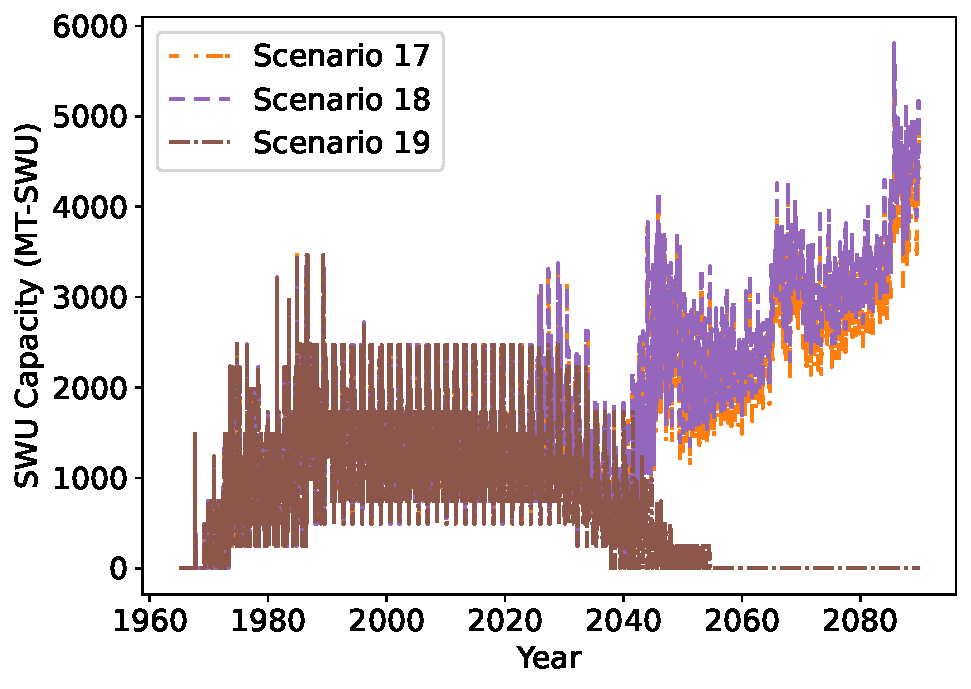
\includegraphics[width=\textwidth]{1percent_recycle_swu.pdf}
        \caption{Monthly SWU capacity required to produce 
        enriched uranium for all reactors between 2025-2090.}
        \label{fig:1percent_recycle_swu_all}
    \end{subfigure}
    \hfill
    \begin{subfigure}[b]{0.45\textwidth}
        \centering
        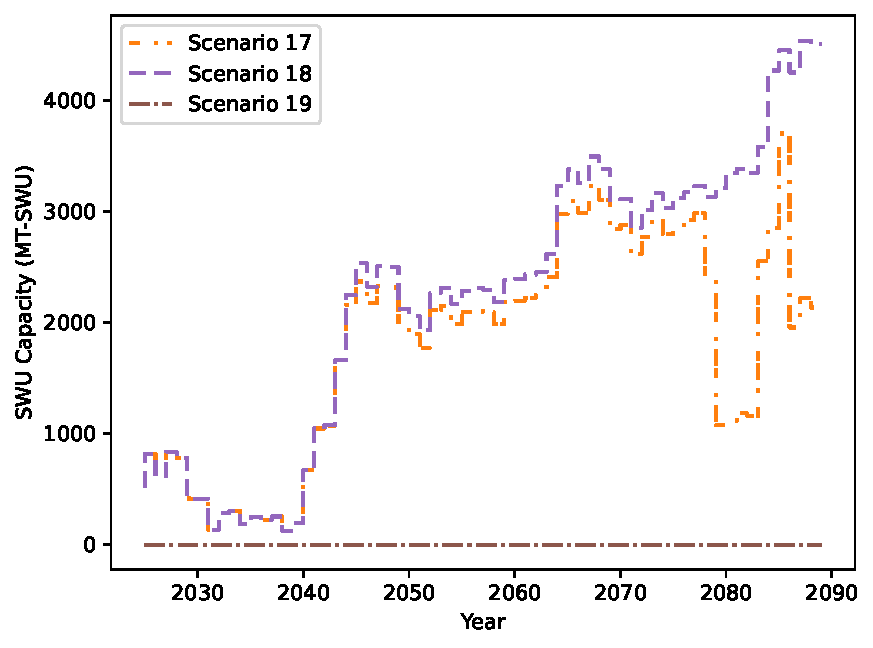
\includegraphics[width=\textwidth]{1percent_recycle_AR_swu.pdf}
        \caption{Monthly SWU capacity required to produce 
        enriched uranium for advanced reactors between 2025-2090.}
        \label{fig:1percent_recycle_swu_AR}
    \end{subfigure}
       \caption{\gls{SWU} capacity required in Scenarios 14-16.}
       \label{fig:1percent_recycle_swu}
\end{figure}

\begin{table}[h!]
    \centering 
    \caption{Metrics for \gls{SWU} capacity required to produce 
    enriched uranium in Scenarios 17-19.}
    \label{tab:s17-19_swu}
    \begin{tabular}{c c c c}
        \hline 
        Scenario & Average (MT-SWU/month) & HALEU Average (MT-SWU/month)
         & Maximum (MT-SWU) \\
        \hline 
        17 & 971.6 & 965.9 & 3,032 \\
        18 & 1,042 & 1,036 & 5,142 \\
        19 & 0 & 0 & 0 \\
        \hline
        
    \end{tabular}
\end{table}

\section{Separated actinide}
The next metric of interest is the separated actinide mass sent 
from the separations facility to the fuel fabrication facility. 
The separated actinide masses include any actinides separated 
from \gls{SNF} (i.e., the uranium, neptunium, plutonium, and 
americium). 
This metric provides context on how much material is available for 
producing plutonium-based fuels, and has implications on 
separations and fabrication facility size needs. Separations facilities 
are deployed starting in 2020, so these results begin in 2020 instead 
of 2025 like the other results. 

\subsection{No growth scenarios}
Figure \ref{fig:nogrowth_recycle_sep_pu} shows the separated plutonium 
masses in Scenarios 14-16. Scenario 16 has the most separated 
plutonium of the three scenarios, which is consistent with the other 
results of these scenarios. Scenarios 14 and 15 have very little 
separated plutonium compared with Scenario 16. The primary reason 
for this large difference is the elements separated out in 
each scenario. In scenario 16, four different actinide elements 
are separated out from the fission products (uranium, neptunium,
plutonium, and americium), but in Scenarios 14 and 15 only plutonium 
is separated out. The inclusion of other elements to separate out 
in Scenario 16 (primarily the uranium, which consists of up to 
93\% of \gls{SNF}), increases the mass of material that can be 
separated out from the \gls{SNF}. 

\begin{figure}[h!]
    \centering
    \begin{subfigure}[b]{0.49\textwidth}
        \centering
        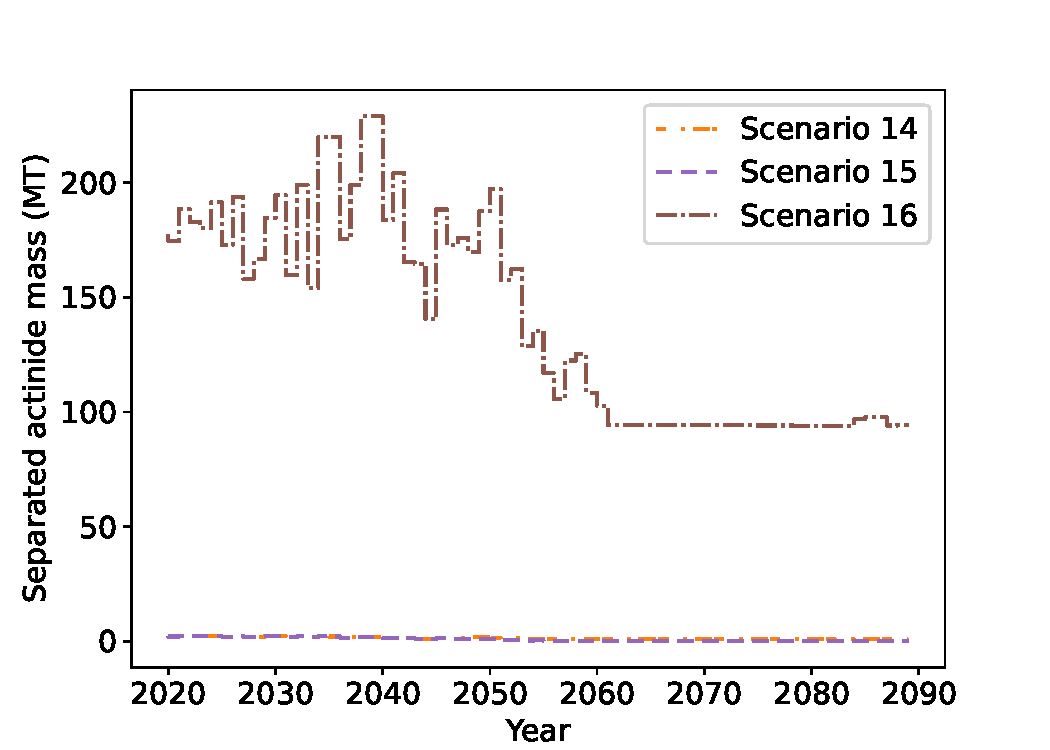
\includegraphics[width=\textwidth]{nogrowth_recycle_sep_pu.pdf}
        \caption{Monthly mass between 2020-2090.}
        \label{fig:nogrowth_recycle_sep_pu_all}
    \end{subfigure}
    \hfill
    \begin{subfigure}[b]{0.49\textwidth}
        \centering
        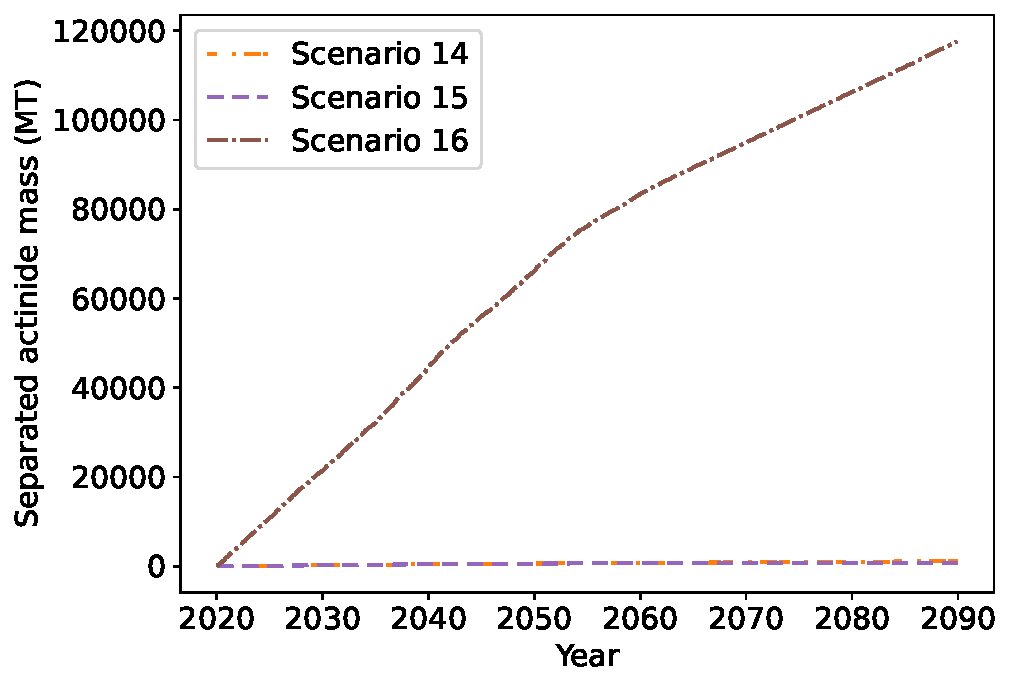
\includegraphics[width=\textwidth]{nogrowth_recycle_sep_pu_cumulative.pdf}
        \caption{Cumulative mass between 2020-2090.}
        \label{fig:nogrowth_recycle_sep_pu_cumulative}
    \end{subfigure}
       \caption{Mass of separated actinides sent from the 
       separations facility to fuel fabrication in Scenarios 14-16.}
       \label{fig:nogrowth_recycle_sep_pu}
\end{figure}

Table \ref{tab:s14-16_sep_pu} reports the metrics of the separated 
plutonium in Scenarios 14-16. All three scenarios experience a 
maximum amount of separated actinides at the same time, in 
December of 2031. This timing corresponds with \gls{SNF} discharged 
from \glspl{LWR} in December of 2025 and fuel from advanced reactors
discharged in October 2031. 

\begin{table}[h!]
    \centering 
    \caption{Metrics of separated actinide masses of between 2020-2090 in 
    Scenarios 14-16.}
    \label{tab:s14-16_sep_pu}
    \begin{tabular}{c c c c}
        \hline 
        Scenario & Average (MT/month) & Maximum (MT) & Cumulative (MT) \\
        \hline
        14 & 1.372 & 4.735 & 1,150\\
        15 & 0.840 & 4.735 & 705.0\\
        16 & 140.1 & 454.3 & 117,584\\
        \hline
    \end{tabular}
\end{table}

From the metrics in Table \ref{tab:s14-16_sep_pu}, the metrics for 
the separated actinide masses in Scenario 16 are two orders of 
magnitude greater than the metrics in Scenarios 14 and 15. The metrics 
for Scenario 16 are also larger than the plutonium-based fuel metrics 
for the scenario in Table \ref{tab:s14-16_mox}. The larger mass 
of separated actinide material than plutonium-based fuels required by 
the reactors drives the lack of enriched uranium to support these 
reactors. The difference between the two material streams stems 
from the reprocessing of uranium from \gls{LWR} fuel, which constitutes 
about 93\% of the \gls{LWR} \gls{SNF}. Therefore, reprocessing 
uranium from \gls{LWR} \gls{SNF} plays an important role in supporting 
this fuel cycle. Between 2060-2090 (after all spent fuel from 
\glspl{LWR} is processed) the \glspl{SFR} require an 
average of 90.3 MT/month of U/TRU fuel, and an average of 95.2 
MT/month of separated actinides. Therefore, the \gls{SFR} could 
still sustain themselves using reprocessed fuel.

Scenario 16 models the reprocessed uranium as being part of 
the fresh reprocessed fuel. Therefore, it is likely that 
fabricating the reprocessed fuel would not need the natural
uranium masses defined in Table \ref{tab:s14-16_natU}. If this 
production method is possible, then the natural uranium needs 
of the fuel cycle would drop to practically zero, further 
emphasizing how a closed fuel cycle can help minimize
natural uranium needs. 

\subsection{1\% growth scenarios}

\begin{figure}[h!]
    \centering
    \begin{subfigure}[b]{0.49\textwidth}
        \centering
        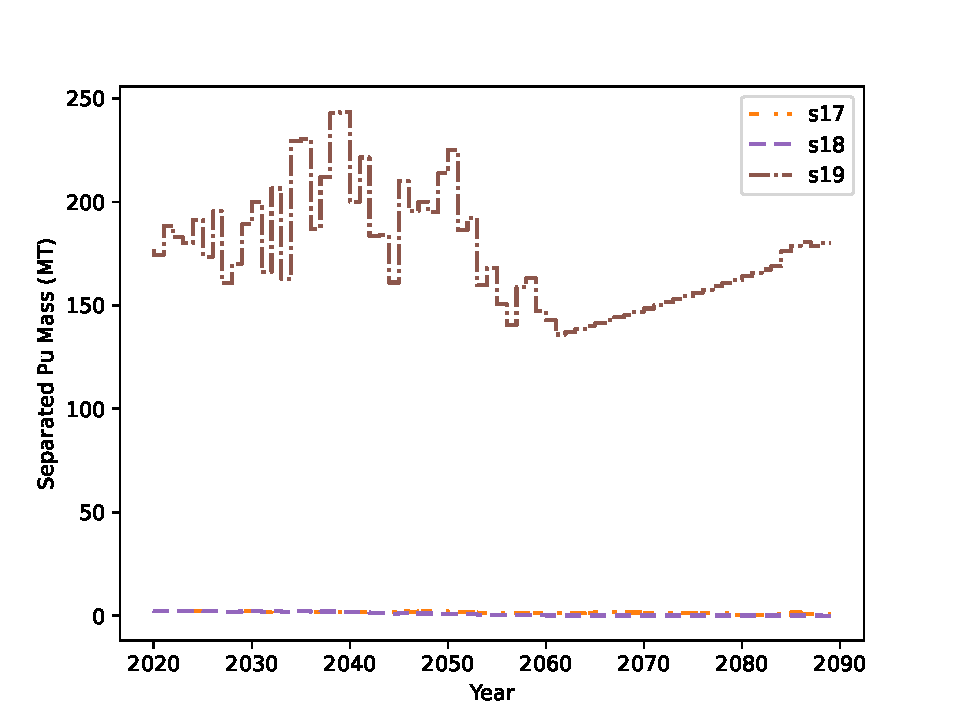
\includegraphics[width=\textwidth]{1percent_recycle_sep_pu.pdf}
        \caption{Separated plutonium mass 
        at each time step between 2020-2090.}
        \label{fig:1percent_recycle_sep_pu_all}
    \end{subfigure}
    \hfill
    \begin{subfigure}[b]{0.49\textwidth}
        \centering
        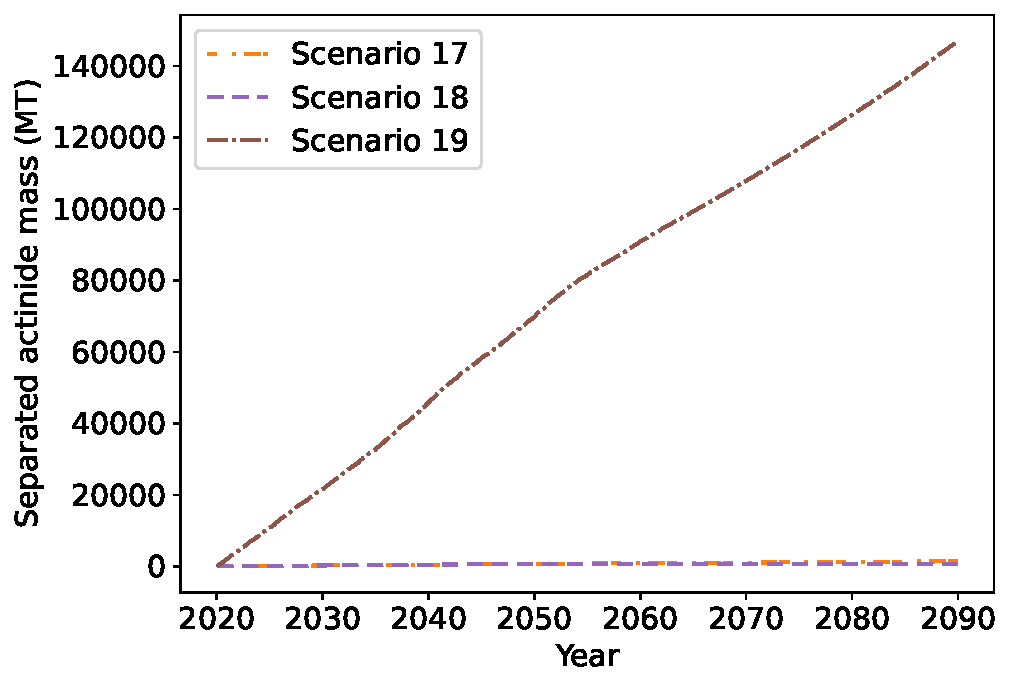
\includegraphics[width=\textwidth]{1percent_recycle_sep_pu_cumulative.pdf}
        \caption{Cumulative mass of separated plutonium 
        at each time step between 2020-2090.}
        \label{fig:1percent_recycle_sep_pu_cumulative}
    \end{subfigure}
       \caption{Separated plutonium masses in Scenarios 17-19.}
       \label{fig:1percent_recycle_sep_pu}
\end{figure}

\begin{table}[h!]
    \centering 
    \caption{Mass of separated plutonium between 2020-2090 in Scenarios 
    17-19.}
    \label{tab:sep_pu_17-19}
    \begin{tabular}{c c c c}
        \hline 
        Scenario & Average (MT/month) & Maximum (MT) & Cumulative (MT) \\
        \hline
        17 &  &  & \\
        18 &  &  & \\
        19 &  &  & \\
        \hline
    \end{tabular}
\end{table}


\section{Spent nuclear fuel and high level waste}
This section provides the results of the \gls{SNF} and \gls{HLW} sent 
to disposal in the closed fuel cycles. The once-through scenario 
results only defined the \gls{SNF} sent for disposal because all 
of the materials needing disposal in those scenarios are \gls{SNF}. 
With the addition of the separation step, the \gls{SNF} discharged 
from reactors gets separated into two different material streams, 
one of the separated plutonium and one of \gls{HLW} that is sent 
for disposal.

\subsection{No growth scenarios}
This section presents the results of the \gls{SNF} and 
\gls{HLW} masses that are sent for disposal in a 
material sink in the no growth recycle scenarios. 

\subsubsection{Spent nuclear fuel}
Figure \ref{fig:nogrowth_recycle_snf} shows the monthly and 
cumulative masses of advanced reactor \gls{SNF} disposed of 
in Scenarios 14-16. In Scenario 14 only the spent \gls{MOX} 
fuel is disposed of, in Scenario 15 the spent \gls{MOX} as 
well as the spent \gls{MMR} and Xe-100 fuels are disposed of, 
and no \gls{SNF} is disposed of in Scenario 16. The disposal of 
\gls{MMR} \gls{SNF} in Scenario 15 leads to the single times 
with larger disposal masses, because of the single-batch 
fueling scheme of the \gls{MMR}. 

\begin{figure}[h!]
    \centering
    \begin{subfigure}[b]{0.49\textwidth}
        \centering
        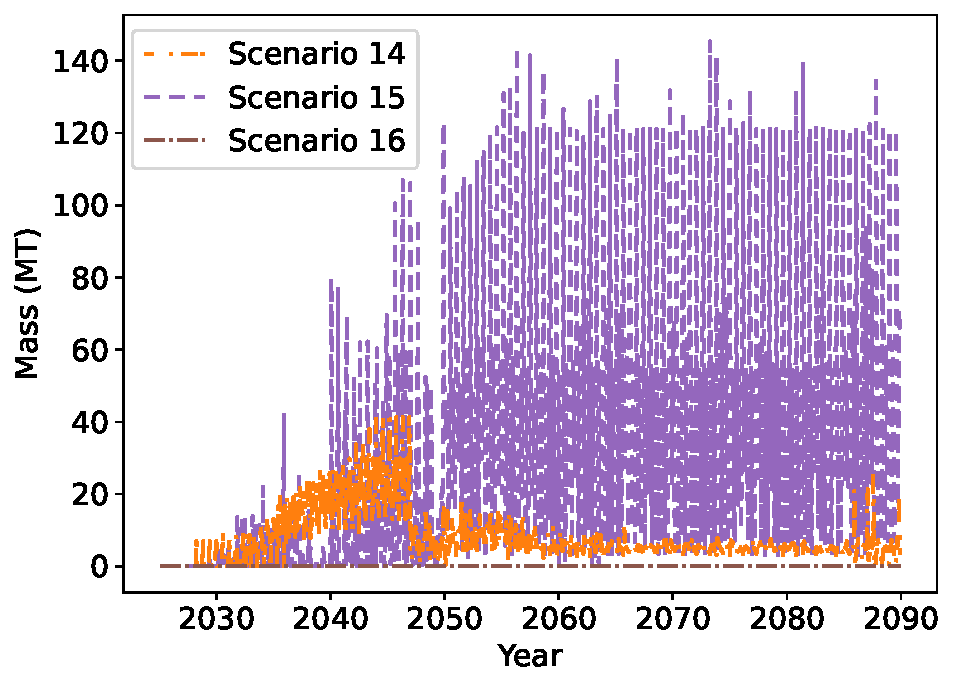
\includegraphics[width=\textwidth]{nogrowth_recycle_snf.pdf}
        \caption{Monthly mass sent for disposal 
        at each time step between 2025-2090.}
        \label{fig:nogrowth_recycle_snf_all}
    \end{subfigure}
    \hfill
    \begin{subfigure}[b]{0.49\textwidth}
        \centering
        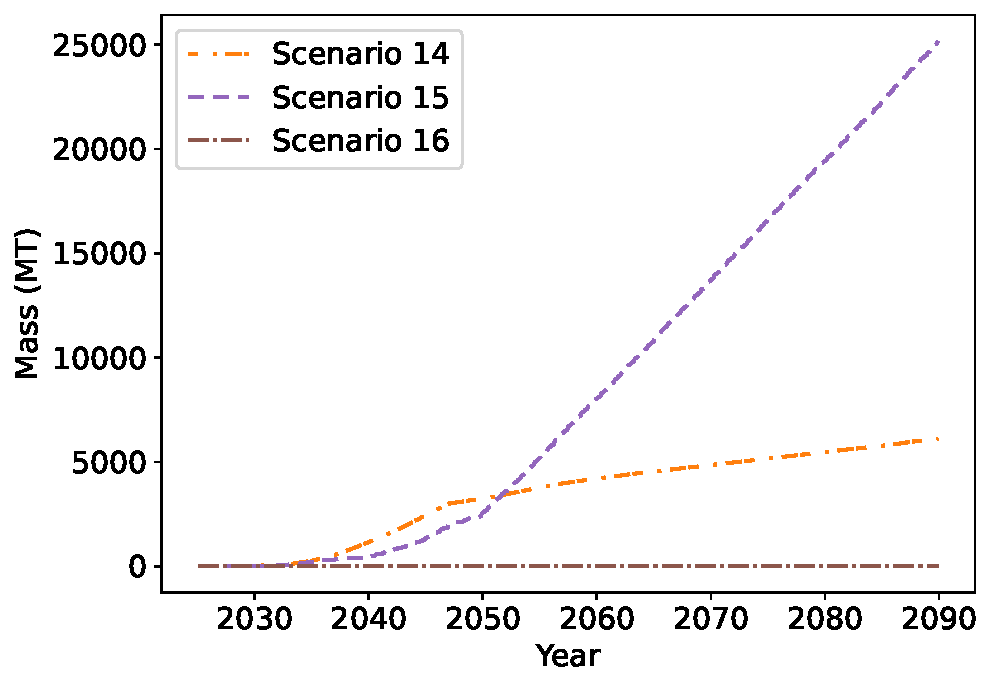
\includegraphics[width=\textwidth]{nogrowth_recycle_snf_cumulative.pdf}
        \caption{Cumulative mass sent for disposal 
        at each time step between 2025-2090.}
        \label{fig:nogrowth_recycle_snf_cumulative}
    \end{subfigure}
       \caption{\gls{SNF} disposed of in Scenarios 14-16.}
       \label{fig:nogrowth_recycle_snf}
\end{figure}

Table \ref{tab:s14-16_snf} reports the metrics for the \gls{SNF} disposal 
in Scenarios 14-16. Based on these values and the results in 
Figure \ref{fig:nogrowth_recycle_snf}, including more fuel for 
reprocessing can greatly reduce the mass of \gls{SNF}. All three of 
these scenarios have a cumulative \gls{SNF} mass smaller than 
that of all of the once-through scenarios. Additionally, 
the \gls{SNF} from advanced reactors in all three of these scenarios 
is less than the 70,000 MT limit for Yucca Mountain. The reduction in 
\gls{SNF} mass compared with the once-through scenarios highlights 
an advantage of closed fuel cycles. 

\begin{table}[h!]
    \centering 
    \caption{Mass of SNF disposed of between 2025-2090 in 
    Scenarios 14-16.}
    \label{tab:s14-16_snf}
    \begin{tabular}{c c c c}
        \hline 
        Scenario & Average (MT/month) & Maximum (MT) & Cumulative (MT) \\
        \hline
        14 & 7.835 & 41.33 & 6,103\\
        15 & 32.29 & 145.4 & 25,153 \\
        16 & 0 & 0 & 0 \\
        \hline
    \end{tabular}
\end{table}

\subsubsection{High level waste}
Finally, Figure \ref{fig:nogrowth_recycle_hlw} shows the 
\gls{HLW} masses for disposal in Scenarios 14-16. Scenario 
14 results in the most \gls{HLW}, because more 
material is reprocessed in this scenario than in Scenario 15, 
and less actinide material is separated out than in 
Scenario 16. The \gls{HLW} mass in Scenario 15 reaches a 
near-zero level around 2060, because all of the \gls{LWR} 
\gls{SNF} is reprocessed by this time which leaves only
the VOYGR \gls{SNF} available for reprocessing. A 
maximum of 7 VOYGRs are deployed at a time in Scenario 
15, so there is very little material reprocessed and 
little \gls{HLW} generated after 2060. 

\begin{figure}[h!]
    \centering
    \begin{subfigure}[b]{0.49\textwidth}
        \centering
        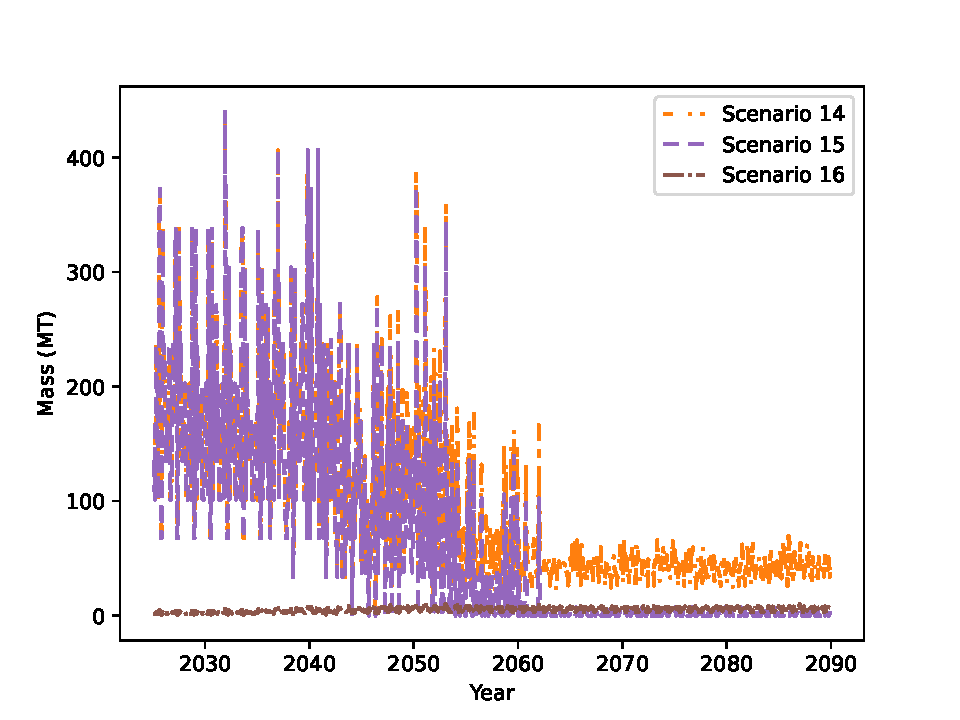
\includegraphics[width=\textwidth]{nogrowth_recycle_hlw.pdf}
        \caption{Monthly mass sent for disposal 
        at each time step between 2025-2090.}
        \label{fig:nogrowth_recycle_hlw_all}
    \end{subfigure}
    \hfill
    \begin{subfigure}[b]{0.49\textwidth}
        \centering
        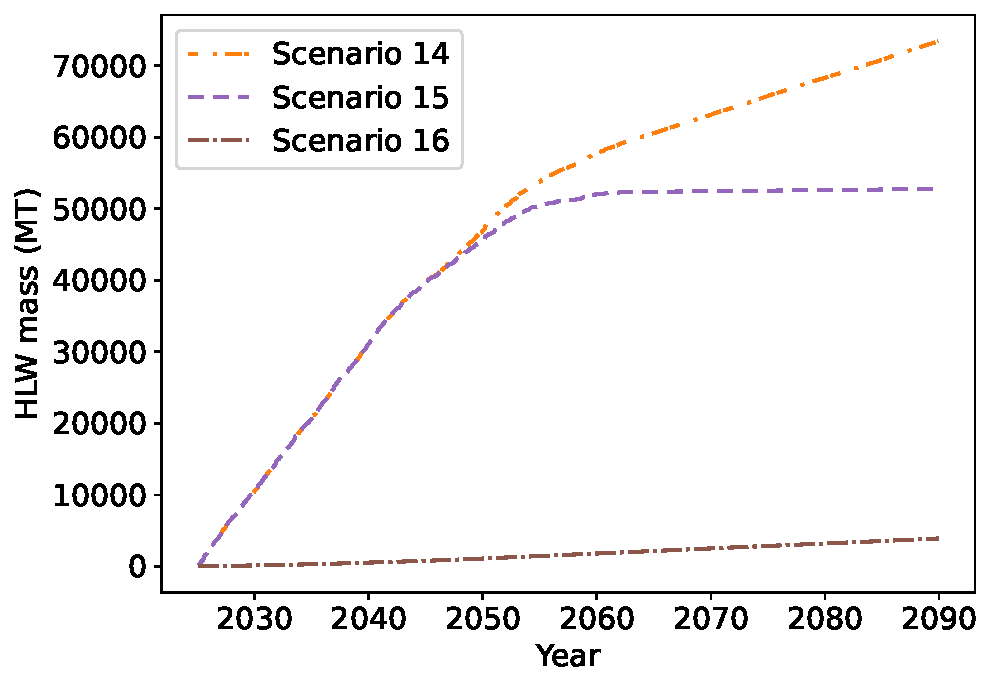
\includegraphics[width=\textwidth]{nogrowth_recycle_hlw_cumulative.pdf}
        \caption{Cumulative mass sent for disposal 
        at each time step between 2025-2090.}
        \label{fig:nogrowth_recycle_hlw_cumulative}
    \end{subfigure}
       \caption{Mass of \gls{HLW} disposed of in Scenarios 14-16.}
       \label{fig:nogrowth_recycle_hlw}
\end{figure}

Table \ref{tab:s14-16_hlw} reports the metrics for the \gls{HLW} 
in Scenarios 14-16. Scenario 16 generates very little 
\gls{HLW} because the actinide material separated out 
comprises most of the mass of the waste material. The \gls{HLW} 
masses for Scenarios 14 and 15 are larger than the \gls{SNF} 
masses for these scenarios, and are larger than the \gls{SNF} 
masses of the no growth, once-through scenarios. The increase 
comes from the inclusion of \gls{LWR} \gls{SNF} for reprocessing 
in these scenarios. Including this \gls{SNF} increases the 
disposed material mass because this metric is not solely focused 
on material from the advanced reactors. The average for 
Scenario 14 is similar to the average \gls{SNF} disposed of 
between 2025-2055 in Scenario 1 (94.27 MT/month), but these 
values consider different time frames. 

\begin{table}[h!]
    \centering 
    \caption{Mass of HLW disposed of between 2025-2090 in 
    Scenarios 14-16.}
    \label{tab:s14-16_hlw}
    \begin{tabular}{c c c c}
        \hline 
        Scenario & Average (MT/month) & Maximum (MT) & Cumulative (MT) \\
        \hline
        14 & 94.21 & 440.2 & 73,389\\
        15 & 67.73 & 440.2 & 52,764\\
        16 & 5.011 & 10.09 & 3,903\\
        \hline
    \end{tabular}
\end{table}

The \gls{HLW} in each of these scenarios has a different 
composition than the \gls{SNF}, but both waste streams 
still require a geologic repository for final 
disposal. Therefore, both the \gls{SNF} and \gls{HLW} 
masses must be considered for evaluating repository 
capacities. The \gls{HLW} in Scenario 14 is more than 
the 70,000 MT limit of Yucca Mountain, so a second 
repository would be needed to disposal of both waste 
streams. The \gls{SNF} and \gls{HLW} materials in 
Scenario 15 sum to 77,917 MY, meaning that a second 
repository would be needed to support this scenario 
as well. These material streams sum to 3,903 MT in 
Scenario 16, which means that the Yucca Mountain 
limit of 70,000 MT would be sufficient to support this 
scenario. 


\subsection{1\% growth scenarios}
This section presents the results of the \gls{SNF} and 
\gls{HLW} masses that are sent for disposal in a 
material sink in the 1\% growth recycle scenarios. 
\subsubsection{Spent nuclear fuel}

\begin{figure}[h!]
    \centering
    \begin{subfigure}[b]{0.49\textwidth}
        \centering
        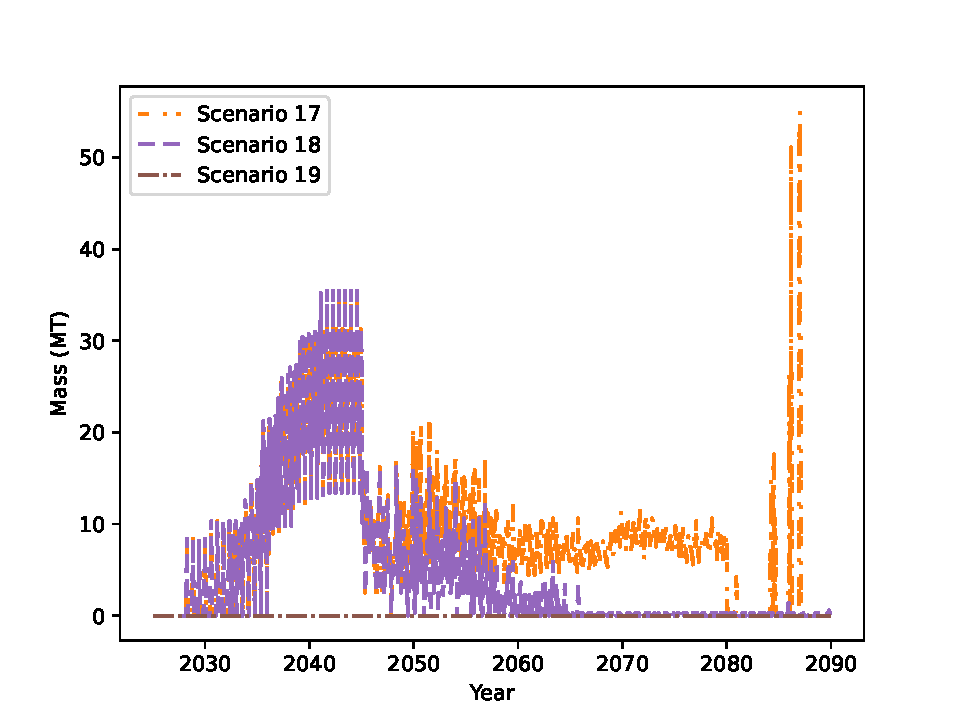
\includegraphics[width=\textwidth]{1percent_recycle_snf.pdf}
        \caption{Monthly mass of SNF sent for disposal 
        at each time step between 2025-2090.}
        \label{fig:1percent_recycle_snf_all}
    \end{subfigure}
    \hfill
    \begin{subfigure}[b]{0.49\textwidth}
        \centering
        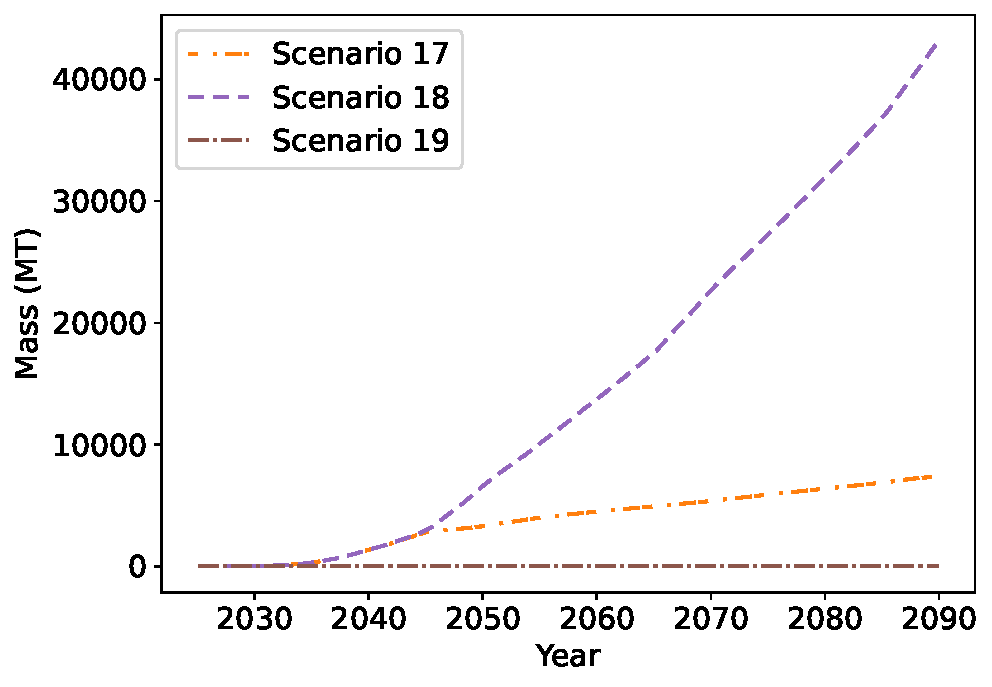
\includegraphics[width=\textwidth]{1percent_recycle_snf_cumulative.pdf}
        \caption{Cumulative mass of SNF sent for disposal 
        at each time step between 2025-2090.}
        \label{fig:1percent_recycle_snf_cumulative}
    \end{subfigure}
       \caption{\gls{SNF} disposed of in Scenarios 17-19.}
       \label{fig:1percent_recycle_snf}
\end{figure}

\begin{table}[h!]
    \centering 
    \caption{Mass of SNF disposed of between 2025-2090 in 
    Scenarios 17-19.}
    \label{tab:snf_17-19}
    \begin{tabular}{c c c c}
        \hline 
        Scenario & Average (MT/month) & Maximum (MT) & Cumulative (MT) \\
        \hline
        17 & & & \\
        18 & & & \\
        19 & & & \\
        \hline
    \end{tabular}
\end{table}


\subsubsection{High level waste}

\begin{figure}[h!]
    \centering
    \begin{subfigure}[b]{0.49\textwidth}
        \centering
        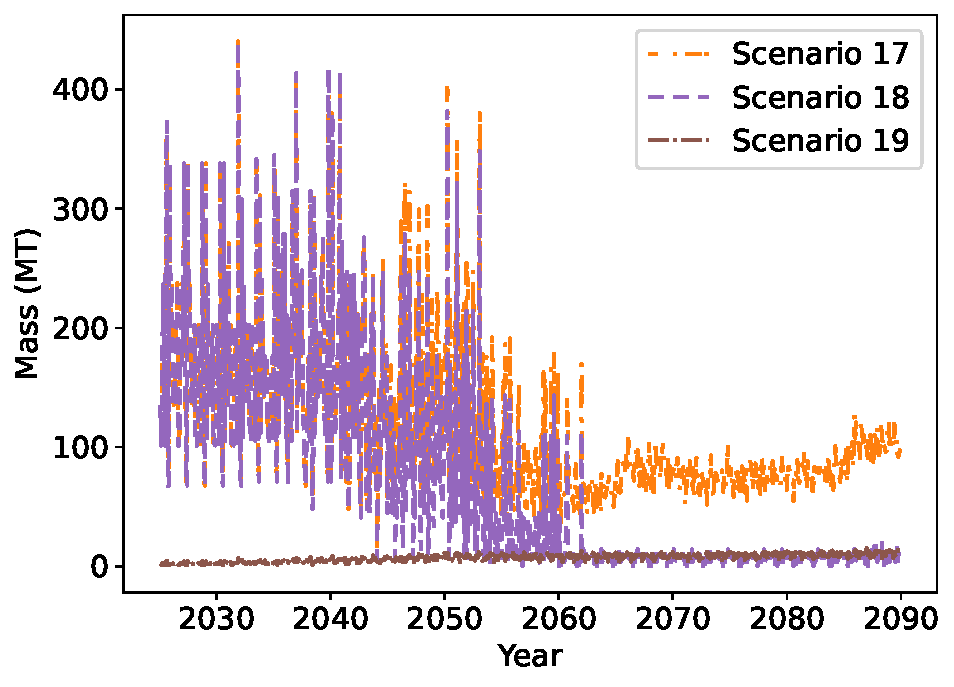
\includegraphics[width=\textwidth]{1percent_recycle_hlw.pdf}
        \caption{Monthly mass of HLW sent for disposal 
        at each time step between 2025-2090.}
        \label{fig:1percent_recycle_hlw_all}
    \end{subfigure}
    \hfill
    \begin{subfigure}[b]{0.49\textwidth}
        \centering
        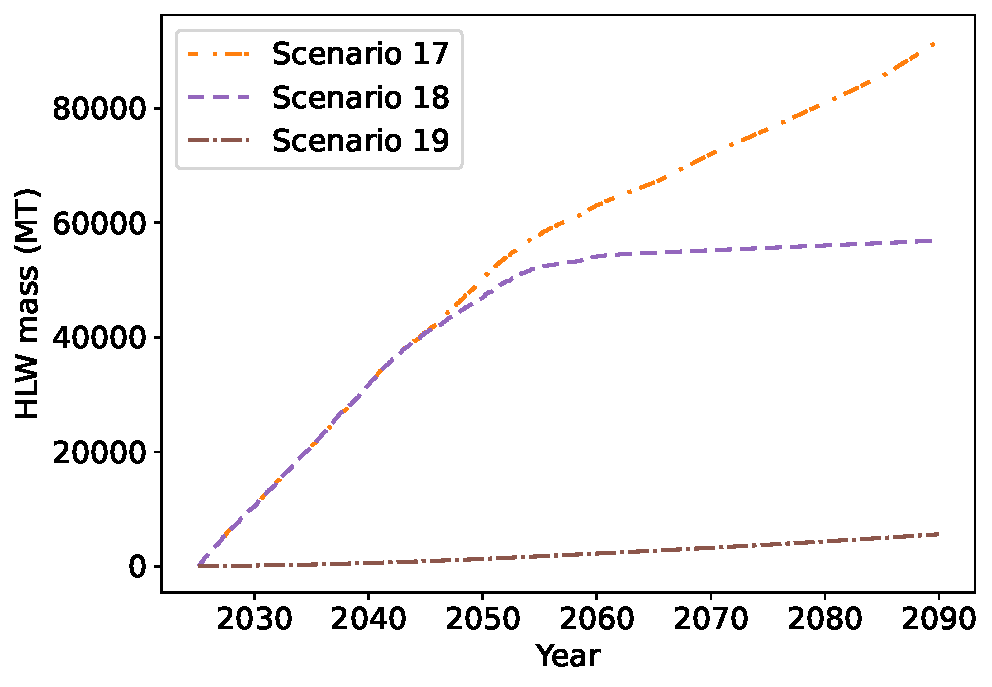
\includegraphics[width=\textwidth]{1percent_recycle_hlw_cumulative.pdf}
        \caption{Cumulative mass of HLW sent for disposal 
        at each time step between 2025-2090.}
        \label{fig:1percent_recycle_hlw_cumulative}
    \end{subfigure}
       \caption{\gls{HLW} disposed of in Scenarios 17-19.}
       \label{fig:1percent_recycle_hlw}
\end{figure}

\begin{table}[h!]
    \centering 
    \caption{Mass of HLW disposed of between 2025-2090 in 
    Scenarios 17-19.}
    \label{tab:hlw_17-19}
    \begin{tabular}{c c c c}
        \hline 
        Scenario & Average (MT/month) & Maximum (MT) & Cumulative (MT) \\
        \hline
        17 & & & \\
        18 & & & \\
        19 & & & \\
        \hline
    \end{tabular}
\end{table}
